% Use the University of Michigan thesis class.
\documentclass[letterpaper,12pt,oneside]{report}
\RequirePackage{times}
\usepackage{rac}


\newcommand{\MYIF}{\textbf{if }}
\newcommand{\MYELSE}{\textbf{else }}
\newcommand{\MYRETURN}{\textbf{return }}
\newcommand{\AlgBox}[1]{{\framebox[1.2\width]{\textbf{#1}}}}
\newcommand{\BULLET}{\vspace{+.05in} \noindent $\bullet$ \hspace{+.12in}}

\newcommand{\firefly}{$\sf\small{Firefly}$\xspace}	
\newcommand{\boldfirefly}{\textbf{Firefly}\xspace}
\newcommand{\bigfirefly}{Firefly\xspace}

\newcommand{\lime}{$\sf\small{LIME}$\xspace}	
\newcommand{\boldlime}{\textbf{LIME}\xspace}
\newcommand{\biglime}{LIME\xspace}
\newcommand{\xing}[1]{{\color{blue}\textit{#1}}}

\usepackage{epsfig,xspace,xspace,color,multirow,endnotes}
\usepackage{graphicx,amssymb,amsmath,endnotes}
\usepackage{array,colortbl,booktabs}
\usepackage{times}
\usepackage{subfigure}
\usepackage{algorithm}
\usepackage{algorithmic}
\usepackage{amsthm}
\usepackage{url}
\usepackage{hyperref}
\usepackage{breakurl}
\usepackage{wasysym, pifont}
\usepackage{gensymb}
\usepackage{tabularx}
\usepackage{caption}

\usepackage{setspace}    % Allows you to specify the line spacing
\doublespacing           % \onehalfspacing for 1.5 spacing, \doublespacing for 2.0 spacing.

\def\UrlBreaks{\do\A\do\B\do\C\do\D\do\E\do\F\do\G\do\H\do\I\do\J
\do\K\do\L\do\M\do\N\do\O\do\P\do\Q\do\R\do\S\do\T\do\U\do\V
\do\W\do\X\do\Y\do\Z\do\[\do\\\do\]\do\^\do\_\do\`\do\a\do\b
\do\c\do\d\do\e\do\f\do\g\do\h\do\i\do\j\do\k\do\l\do\m\do\n
\do\o\do\p\do\q\do\r\do\s\do\t\do\u\do\v\do\w\do\x\do\y\do\z
\do\.\do\@\do\\\do\/\do\!\do\_\do\|\do\;\do\>\do\]\do\)\do\,
\do\?\do\'\do+\do\=\do\#}


\newcommand{\etc}{\emph{etc.}\xspace}
\newcommand{\ie}{\emph{i.e.,}\xspace}
\newcommand{\eg}{\emph{e.g.,}\xspace}
\newcommand{\etal}{\emph{et al.}\xspace}
\newcommand{\wrt}{\emph{w.r.t.}\xspace}
\newcommand{\mycomment}[1]{{\color{red}[\textsf{#1}]}}

\newcommand{\DCH}{$\sf\small{DCH}$}
\newcommand{\DCHH}{$\sf\small{DCH}$ }
\newcommand{\FACH}{$\sf\small{FACH}$}
\newcommand{\FACHH}{$\sf\small{FACH}$ }
\newcommand{\IDLE}{$\sf\small{IDLE}$}
\newcommand{\IDLEE}{$\sf\small{IDLE}$ }
\newcommand{\RC}{$\small{\textbf{\texttt{RRC\_CONNECTED}}}\normalsize$\xspace}
\newcommand{\RI}{$\small{\textbf{\texttt{RRC\_IDLE}}}\normalsize$\xspace}

\newcommand{\MR}[1]{\multirow{2}{*}{#1}}
\newcommand{\hd}[1]{\small{\textbf{\texttt{#1}}}\normalsize}
\newcommand{\hds}[1]{\small{\textbf{\texttt{#1}}}}

\newcommand{\ISP}{$\sf\small{ISP}$}
\newcommand{\ISPP}{$\sf\small{ISP}$ }

\theoremstyle{definition} \newtheorem{apitest}{Test}
\newcommand{\YY}{\CIRCLE}
\newcommand{\NN}{\Circle}
\newcommand{\YN}{\RIGHTcircle}
\newcommand{\XX}{\ding{53}}

\begin{document}

\titlepage{Characterizing and Optimizing Emerging Mobile Applications From the System Perspective}{Xing Liu}{Doctor of Philosophy}
{Computer Science and Engineering}{2020}
{Professor Zhi-Li Zhang, Chair \\
Assistant Professor Feng Qian \\
Assistant Professor Evan Suma Rosenberg \\
Principal Inventive Scientist Dr. Bo Han, AT\&T Labs -- Research}

\copyrightpage{Xing Liu}

\initializefrontsections

% Dedication
\dedicationpage{\emph{To my family.}}

% Acknowledgments
%\acknowledgments[6]{
\startacknowledgementspage
I would like to thank many people who helped me during this long journey of Ph.D. study...
%}
\label{ACKNOWLEDGEMENTS}



\tableofcontents     % Required
\listoffigures       % Required if there is more than one figure
\listoftables        % Required if there is more than one table

\startabstractpage{
Characterizing and Optimizing Emerging Mobile Applications From the System Perspective}{Xing Liu}{Chair: Zhi-Li Zhang}
The past few years have witnessed exciting mobile technologies advances: high-speed LTE access has become a norm, mobile devices are unprecedentedly powerful, VR/AR has eventually stepped out of the lab, wearable devices are waving computing into our daily lives, \emph{etc}.
 Although above remarkable achievements have boosted the emergence of various novel mobile applications, there still remains three major challenges for researchers, developers as well as the mass mobile users. First, emerging mobile applications are still relatively new to the commercial market, and the research community lacks a thorough understanding of their ecosystem. 
 Second, emerging mobile applications pose stringent requirements for computing and networking capability, leaving their quality of experience (QoE) suffers in the presence of constrained mobile CPU/GPU and challenging network condition. 
 Third, emerging mobile applications are operating under tight battery budget, however they often time incur non-trivial energy overhead. 
 My dissertation is dedicated to address above challenges identified in three representative emerging mobile usage scenarios: \emph{360\degree{} live video}, \emph{Virtual Reality(VR)}, and \emph{wearable applications}. 
 The goal is to uncover their unique characteristics by comprehensive measurements, propose optimizations towards their major inefficiencies, and implement empirical system to improve the QoE.
  Specifically, we designed and implemented \lime (LIve video MEasurement platform), a generic and holistic system allowing researchers to conduct crowd-sourced measurements with 360\degree{} live video streaming. We utilized \lime to perform a first study of personalized 360\degree{} live video streaming on popular commercial platforms. \lime reveals significant network utilization inefficiencies across different streaming platforms that were previously ignored. Our findings suggested that bringing viewport-adaptive streaming into 360\degree{} live video could significantly improve viewer side QoE in the presence of challenging network conditions. 
 Inspired by the 360\degree{} video measurement study, we further studied generic VR. We designed, implemented, and evaluated an untethered multi-user VR system, called \firefly, that supports more than 10
 users to simultaneously enjoy high-quality VR content using a
 single commodity server, a single WiFi access point (AP), and commercial
 off-the-shelf (COTS) mobile devices. \firefly employed
 a series of innovations to adapt to the stringent networking and rendering requirements of supporting high quality VR on commodity smartphones. Our prototype of \firefly demonstrated, for
 the first time, the feasibility of supporting 15 mobile VR users
 at 60 FPS using COTS smartphones and a single AP/server.
 We also performed in-depth characterization of emerging wearable applications. In particular. We conducted an IRB-approved
 measurement study involving 27 Android smartwatch users. Using
 a 106-day dataset collected from our participants, we performed indepth
 characterization of three key aspects of smartwatch usage “in
 the wild”: usage patterns, energy consumption, and network traffic.
 Our findings revealed root causes for wearables' shortened battery life and we proposed optimizations to further improve the energy efficiency of smartwatches. 
\label{Abstract}


\startthechapters

\chapter{Introduction} \label{chap:intro}

Emerging mobile applications have experienced a bloom in the recent years particularly thanks to the growing diversity and capability of mobile gadgets, namely handheld, head mounted, and wearable devices. As reported by Statista~\cite{VRARusers}, the total number of VR/AR users has doubled from 60 millions to 125 millions over the past 4 years, and will continue to show steady growth in the future. Also, wearable device usage is becoming more and more common and its user base is expanding at a remarkable pace. As documented~\cite{wearableusers}, the amount of wearable device users has increased 124\% compared with 4 years ago, with the total number reaching 57 millions as of 2019. Despite the popularity of emerging mobile devices and their applications, there remain three major challenges associated with developers and their mass users.

First, we lack a systematic understanding of the ecosystem of emerging mobile applications. Novel streaming service such as 360\degree{} live video allows users to enjoy real-time \emph{panoramic} content from their smartphones, tablets, even web browsers. Although being increasingly popular, the service is still relatively new to the commercial market, and we are unfamiliar with its live characteristics such as bandwidth consumption, streaming quality, latency, stalls, \emph{etc}. Also, the high data rate of panoramic content makes its QoE being more sensitive to challenging network condition. For example, in our user study we found that more than 65\% of the 360\degree{} live viewing sessions produce a lower perceived image quality than 480P. Therefore, QoE of 360\degree{} live video streaming needs to be improved, and a systematic characterization is the first step.

Second, emerging mobile applications such as untethered VR pose stringent requirements for computation and networking, whose capability are often limited in a mobile usage scenario. In particular, today's commodity mobile devices are far from being powerful enough to perform heavy-duty real-time rendering for high-quality VR. A naive solution is to build an real-time offloading model where rendering tasks are distributed to edge server, however previous studies~\cite{boos2016flashback,lai2019furion} indicate that this approach incurs overwhelming bandwidth usage by streaming the rendered content to mobile clients. Another key challenge is multi-user scalability, which calls for strategic decisions of splitting the client-server
workload, as well as scalable approaches for rendering and distributing
the content.

Third, emerging mobile applications, for example wearable apps, are operating under tight energy budget. Based on our findings, the battery capacity of a typical smartwatch is only 10\% $\sim$ 25\% compared to that of smartphones. The average standby time for popular off-the-shelf smartwatches is only around 40 hours, much lesser compared with traditional watches. Practicing good energy efficiency is especially important for smartwatches given its small battery capacity. In literature, very few efforts have been made on understanding the energy profile and usage behavior of smartwatch, not to mention optimizing its energy efficiency.

My thesis is dedicated to address above challenges for three representative emerging mobile applications which are \emph{360\degree{} live video}, \emph{untethered VR}, and \emph{wearable applications}. The goal is to \emph{uncover their unique characteristics, propose optimizations towards major inefficiencies, and implement empirical system to improve the QoE}. Here I elaborate the contributions of my dissertation in the following three sections.


\section{\emph{Measuring the State of the Art}: Understanding Commercial 360\degree{} Live Video Streaming Services}

%summarize problem.
%summarize approach.
%summarize contributions.

Personalized 360\degree{} live video streaming is an increasingly popular mobile service that allows a broadcaster to share panoramic videos in real time with worldwide viewers. Compared to video-on-demand (VOD) streaming, experimenting with live broadcast is harder due to its intrinsic live nature, the need for worldwide viewers, and a more complex data collection pipeline. In addition, 360\degree{} live video requires much higher bandwidth to provide the same perceived quality as regular
video streaming. It has more
stringent QoE requirements to prevent VR
motion sickness, and it incurs higher workload across all entities:
\emph{broadcasters}, \emph{streaming infrastructure}, and \emph{viewers}.

We provided insights for today’s commercial 360\degree{} live video streaming services. The overall goals are two-fold. First, due to
a lack of measurement tools, we develop a measurement system
called \lime (LIve video MEasurement platform), which allows researchers
to conduct crowd-sourced measurements on commercial
or experimental live streaming platforms. Second, we present, to
the best of our knowledge, a first study of 360\degree{} personalized live
video streaming on commercial platforms. We select YouTube and
Facebook as the target platforms given their popularity.

To summarize, we made the following contributions. First, the \lime infrastructure itself is a generic, holistic, and crowd-sourced measurement system.
LIME can be used in conjunction with the majority of today’s commercial live video streaming platforms. 
Second, leveraging \lime, we collected data from 548 users in 35 countries who have watched more than 4,000 minutes of 360\degree{} live videos. We use this dataset to examine 360\degree{} live video streaming performance in the wild.
Third, we quantified the impact of viewport adaptiveness on 360\degree{} live video streaming, and identified inefficiencies of commercial platforms that diminish the benefits of viewport adaptiveness.


\section{\emph{Improving the Quality of Experience}: Engineering High Quality Untethered Multi-user VR over Enterprise Wi-Fi}
Virtual Reality has registered numerous applications. Despite the recent trend of ``cutting the cord'' and making VR untethered over wireless networks, providing immersive user experience on mobile devices still poses numerous challenges. 
The CPU/GPU power of a smartphone is at least one order of magnitude lower than its desktop counterpart~\cite{satyanarayanan2019computing}, not to mention the energy/heat constraints;
the heterogeneity of their computational capabilities should also to be taken into consideration;
stringent network requirements (delay and data rates) of untethered VR can be hardly supported by state-of-the-art wireless networks;
another key challenge is multi-user scalability, which makes above limitations even more urgent. 

We designed, implemented, and evaluated an untethered multi-user VR system, called \firefly, that supports more than 10 users to simultaneously enjoy high-quality VR content using a single commodity server, a single WiFi access point (AP), and commercial off-the-shelf (COTS) mobile devices. 
\firefly employs a series of techniques including offline content preparation,
viewport-adaptive streaming with motion prediction, adaptive
content quality control among users, to name a few, to ensure
good image quality, low motion-to-photon delay, high frame
rate at 60 FPS, scalability with respect to the number of users,
and fairness among users.

\firefly is to our knowledge the first system that can scale
untethered multi-user mobile VR. We make multi-fold contributions:
(1) the design of \firefly, (2) a study of real VR users’ motion, and
(3) our prototype implementation that demonstrates the support of 15 VR 
users at 60 FPS using COTS smartphones and a single AP/server. With emerging
wireless technologies (\emph{e.g.}, 802.11ax and 5G), we believe that \firefly has 
the potential to scale up to even more users.



\section{\emph{Optimizing the Energy Efficiency}: Characterizing Wearable Usage In The Wild}
Smartwatch has become one of the most popular wearable computers on the market. It brings convenience into our daily routine by enabling various interactions such as push notifications, health tracking, voice command, navigation, \emph{etc}.    
Smartwatches are operating under limited energy budget. The battery capacity of a typical smartwatch is only 10\% $\sim$ 25\% compared to that of smartphones.
Charging a watch usually requires special charging dock, making it difficult for users
to charge the watches during the day. It is critical to ensure energy efficient practice for smartwatches since a shortened standby time will undermine user experience.

The very first step towards optimizing smartwatches' energy efficiency is to systematically understand their usage in the wild. To this end, we conducted an IRB-approved measurement study involving 27 Android smartwatch users. Using
a 106-day dataset collected from our participants, we performed in-depth
characterization of three key aspects of smartwatch usage “in
the wild”: usage patterns, energy consumption, and network traffic. 

Our contributions towards optimizing smartwatch energy efficiency can be summarized as follows. First, we developed a automated, lightweight, and self-contained measurement data collection system. The data collection infrastructure is compatible with any smartwatch that runs Android Wear OS. Second, We derived accurate and comprehensive power models for popular commodity Android Wear watches. Third, we performed systematic measurements of smartwatches’ usage
patterns, energy consumption profiles, and network traffic characteristics
using a 106-day dataset collected from 27 users. Based on
our findings, we identified key aspects in the smartwatch ecosystems
that can be further improved, and provided insights towards optimizing energy efficiency.


\section{Thesis Organization}

This dissertation is structured as follows...


\chapter{Background} \label{chap:background}



\section{TBD}


%\chapter{\emph{Measuring the State of the Art}: Understanding Commercial 360\degree{} Live Video Streaming Services} \label{chap:360video}



\section{Introduction}
Personalized 360\degree{} live video streaming is an increasingly popular mobile service that allows a broadcaster to share panoramic videos in real time with worldwide viewers. Compared to video-on-demand (VOD) streaming, experimenting with live broadcast is harder due to its intrinsic live nature, the need for worldwide viewers, and a more complex data collection pipeline. In addition, 360\degree{} live video requires much higher bandwidth to provide the same perceived quality as regular
video streaming. It has more
stringent Quality of Experience (QoE) requirements to prevent VR
motion sickness, and it incurs higher workload across all entities:
\emph{broadcasters}, \emph{streaming infrastructure}, and \emph{viewers}.


We provide insights from today’s commercial live video streaming services. The overall goals are two-fold. First, due to
a lack of measurement tools, we develop a measurement system
called LIME (LIve video MEasurement platform), which allows researchers
to conduct crowd-sourced measurements on commercial
or experimental live streaming platforms. Second, we present, to
the best of our knowledge, a first study of 360\degree{} personalized live
video streaming on commercial platforms. We select YouTube and
Facebook as the target platforms given their popularity.

We begin with developing LIME, a measurement system for live
video streaming. LIME automates the operations of one or multiple
broadcasters so that they can stream pre-recorded videos --
which enables repeatable experiments -- via both commercial (Facebook,
YouTube, Periscope, etc.) and experimental live streaming services.
LIME allows recruiting crowd-sourced viewers via Amazon
Mechanical Turk (AMT)~\cite{amt}, today’s most popular crowd-sourcing
platform. The crowd-sourced viewers are instructed to install a
Chrome extension and watch live video feeds through the platform
under test. The extension collects key performance statistics
while the viewers watch the live videos streamed from broadcasters
under LIME’s control. Note that LIME itself is a generic measurement
system that can work with both 360\degree{} and non-360\degree{} live video
broadcasting on a wide range of streaming platforms.

We leverage LIME to collect crowd-sourced measurement data
from commercial live 360\degree{} video streaming services. Specifically,
we deploy LIME and use AMT to recruit 548 viewers from 35 countries.
Our crowd-sourced viewers watched more than 4,000 minutes
of 360\degree{} live videos on YouTube and Facebook, providing a unique
\emph{viewer-side} dataset. We then conduct a comprehensive measurement
study using this dataset. We make several key observations regarding
live 360\degree{} video streaming on today’s commercial platforms. (1) Overall, the quality is not high, with 34\% (35\%) of YouTube
(Facebook) sessions having an average panoramic quality no higher
than 720p. Because only around 15\% of a panoramic scene is typically
viewed, this translates to a much lower user-perceived quality
comprised between 240p and 360p. (2) Both streaming platforms
are afflicted by long stalls, with 47\% (52\%) of YouTube (Facebook)
sessions stalling for at least 5 seconds per minute. Surprisingly, we
find such stalls are usually not attributed to the network; instead
they are likely caused by the client-side computation/rendering
overhead. (3) We develop a novel methodology for measuring the
broadcaster-to-viewer (B2V) latency, whichwe find to be non-trivial
for both YouTube (median 37.1 seconds) and Facebook (median 18.7
seconds); low-throughput sessions may have B2V latency of up to
5 minutes.

Motivated by our findings, we further leverage
LIME to conduct controlled experiments to measure how \emph{adaptiveness} 
could benefit the viewers and
the broadcaster. On the viewer side, we consider performing
viewport-adaptive streaming where the server only streams content
in the (predicted) viewport of a viewer. We find that performing
viewport-adaptive streaming effectively reduces the video encoding
bitrate by 75\% to 80\%. However, surprisingly, doing so does not
necessarily improve the video quality on Facebook and YouTube
due to several practical issues such as cautious rate adaptation design
and a limited number of quality levels. On the broadcaster
side, we use live videos and real-world cellular uplink traces to
demonstrate the potential of adaptive upload, a unique optimization
for personalized live 360\degree video streaming where the broadcaster
adaptively shrinks the view being uploaded from a full panorama
to smaller regions when the uplink bandwidth is insufficient. This
approach has potentials of significantly reducing the stall duration
(up to 99.9\% reduction in our experimented scenario) and the B2V
latency (up to 38\% reduction).

To summarize, we make the following contributions:
\begin{itemize}
	\item \textbf{The LIME System}. We develop LIME, a generic, holistic,
	and crowd-sourced measurement system for live videos.
	LIME can be used in conjunction with the majority of today’s
	commercial live video streaming platforms.
	\item \textbf{Crowd-sourced Measurement}. Leveraging LIME,
	we collect data from 548 users in 35 countries, and use this
	dataset to examine 360\degree{} live video streaming performance in
	the wild.
	\item \textbf{Controlled Experiments}. We quantify the impact of
	viewport adaptiveness on 360\degree{} live video streaming. We identify
	inefficiencies of commercial platforms that diminish the
	benefits of viewport adaptiveness.
\end{itemize}



\section{LIME Overview}

\begin{figure*}
	\footnotesize
	\begin{center}
		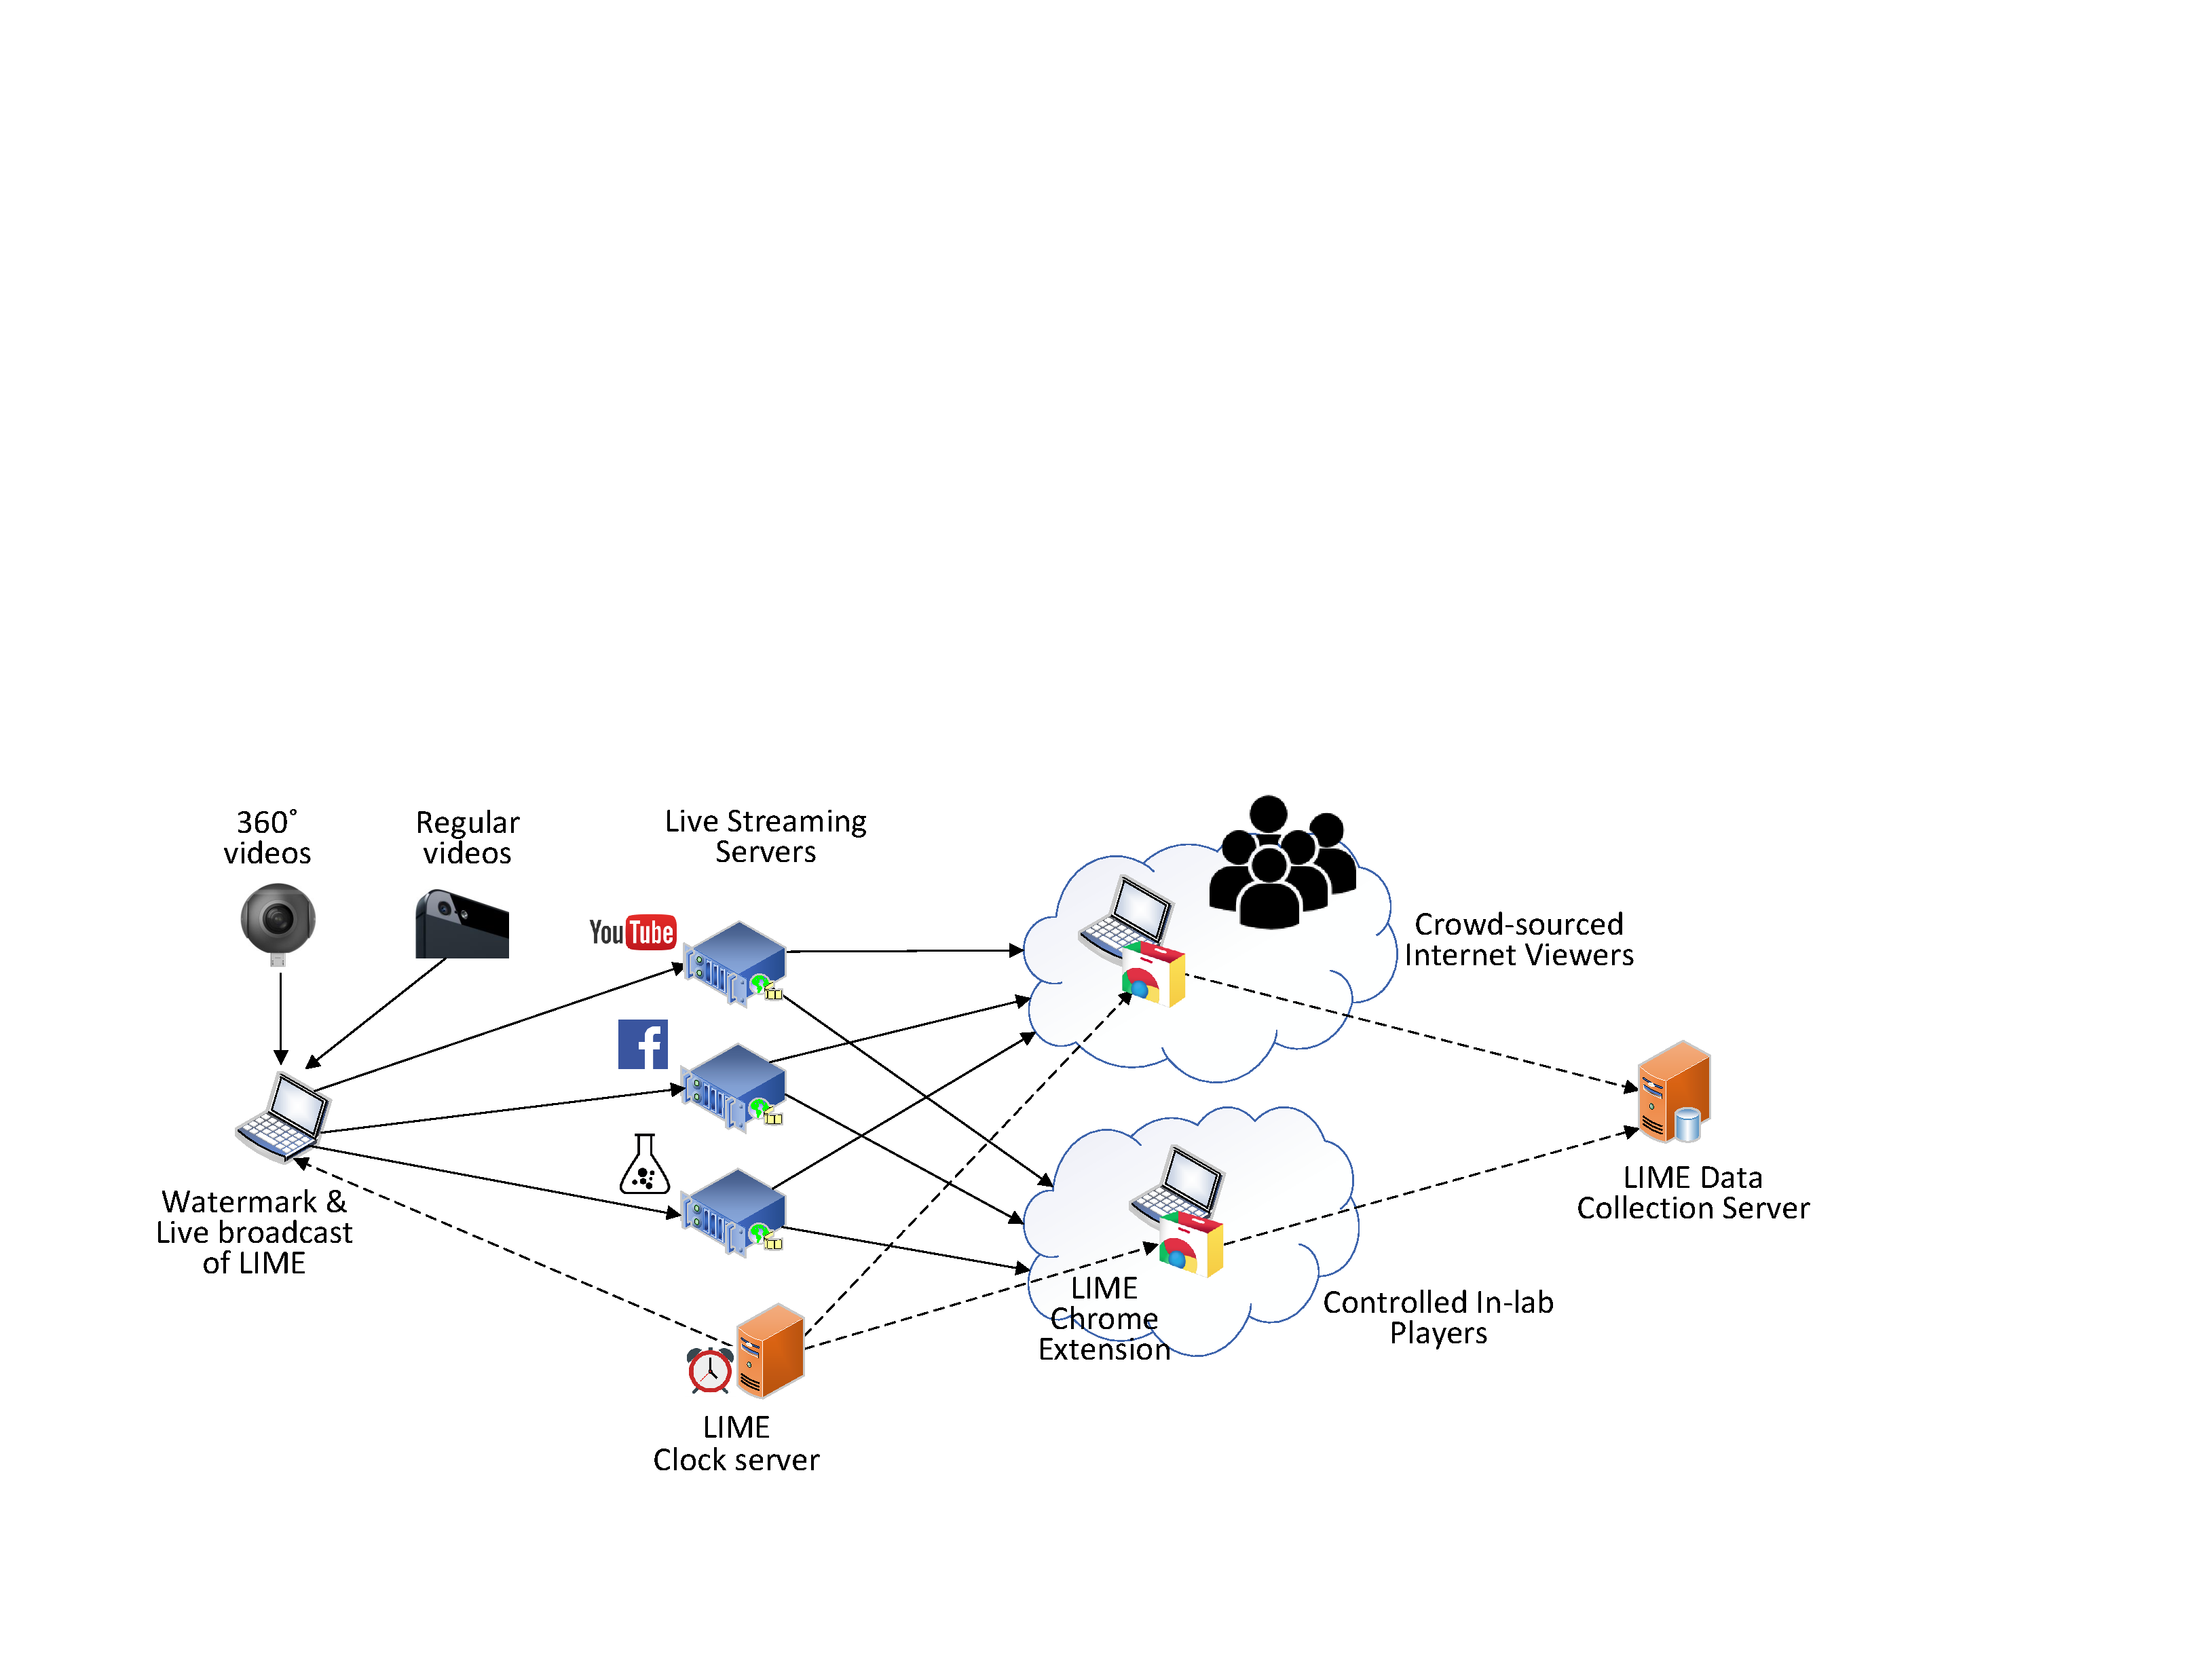
\includegraphics[width=0.9\textwidth]{figs/lime/testbed3.pdf}
	\end{center}
	%\vspace{-.2in}
	%\caption{System for collecting viewer-side performance statistics.}
	\caption{The system architecture of \lime.}
	%\vspace{-.2in}
	\label{fig:testbed}
\end{figure*}

%\mvnote{update figure accordingly}
Figure~\ref{fig:testbed} shows \lime's key components: the \emph{broadcaster}, \emph{streaming servers}, a set of \emph{viewers} (either crowd-sourced viewers or controlled players), the data collection server, and the clock server.
%
The broadcaster is a Linux machine instrumented with Open Broadcaster Software (OBS) Studio~\cite{obs} to broadcast pre-recorded videos to the target streaming servers, either commercial or controlled by the ``experimenter'' \emph{i.e.}, a researcher using \lime for her own studies. Such a ``replay'' approach ensures repeatable experiments.
%
The vast majority, if not all, of popular live streaming services (\eg YouTube, Facebook, Periscope, and Twitch) currently support OBS and can be thus tested via \lime.
%
The experimenter can use either a regular camera to shoot non-360\degree{} videos,
or a panoramic camera (\eg Insta360~\cite{insta360}) to capture 360\degree{} videos.
%
The viewers consist of both \emph{crowd-sourced} Internet viewers and \emph{in-lab} players.  To allow recruiting viewers in a short period of time, we integrate \lime with Amazon Mechanical Turk~\cite{mturk}, a popular crowd-sourcing platform.
%
The experimenter can thus select a number of target viewers (with specific locations/demographics if needed), how many videos they should watch, and their compensation. In-lab players consist of Chrome's instances equipped with \lime's Chrome extension (described next) which are automated via Selenium.\footnote{https://www.seleniumhq.org/}
%\mvnote{I know right know these instances are manually run, but I don't see an issue to integrate with selenium.}

\lime collects viewing statistics using a Google Chrome extension.
%We choose a browser extension because it is agnostic of the live streaming service, \eg commercial or not.
%
We choose a browser extension because it is lightweight, secure, and easy to install.
%agnostic of the live streaming service, \eg commercial or not.
%
Running in the background on the viewer side, the extension collects the following data summarized in Table~\ref{tab:datacollected}: (1) the video playback quality (\eg 720p), (2) stall (\ie rebuffering) events, (3) HTTP request/response headers, (4) user interactions such as dragging the mouse to change the viewport, and (5) periodically captured (every 2 seconds) screenshots of the visible portion of the video.

\begin{table}[]
	\centering
	\small
	\begin{tabular}{l|l|l}
		\multicolumn{1}{c|}{Item}  & \multicolumn{1}{c|}{API/Obj} & \multicolumn{1}{c}{Interval} \\
		\hline
		Video Quality Change & \texttt{HTML Player}     & Event Triggered \\
		Rebuffering Events   & \texttt{HTML Player}     & Event Triggered       \\
		HTTP Req/Res Headers & \texttt{chrome.debugger} & Event Triggered       \\
		User Interactions    & \texttt{HTML Window}     & Event Triggered       \\
		Video Screenshots    & \texttt{chrome.tabs}     & Every 2 Seconds    \\
	\end{tabular}
	\caption{Data items collected by \lime.}
	\label{tab:datacollected}
\end{table}

Finally, Figure~\ref{fig:testbed} shows that \lime further includes two servers under the experimenter's control: a \emph{data collection server} and a \emph{clock server}. The data collection server is the end-point where users' viewing statistics collected by the Chrome extension are uploaded to. The clock server provides synchronized clock readings to both the broadcaster and the viewers, in order to enable accurate measurement of the broadcaster-to-viewer latency. More details will be provided in~\S\ref{sec:b2v}.


\subsection{Measuring the Broadcaster-to-Viewer (B2V) Latency}
\label{sec:b2v_overview}
B2V latency is an important QoE metric for live streaming. We define it as the latency from when a frame leaves the broadcaster to when the frame is consumed by a viewer. A long B2V latency causes lags that are undesirable for real-time live events such as sports. One possible methodology of measuring B2V latency is as follows.
%
The broadcaster watermarks every frame $f$ with a timestamp $t_B(f)$
denoting the time when the frame is generated.
%to leverage timestamps watermarked at the broadcaster, denoted as $t_B$.
When the same frame $f$ is being played, the viewer obtains the current timestamp $t_V(f)$ from the clock server (Figure~\ref{fig:testbed}). Meanwhile, $t_B(f)$ can be extracted from the frame (we use Tesseract OCR~\cite{tesseract-ocr} to perform text recognition on screenshots).
The B2V latency for $f$ is therefore $t_V(f)-t_B(f)$.
%
Note that $t_B(f)$ is obtained from the same clock server as $t_V(f)$.
%
Also note that the originally obtained $t_B(f)$ and $t_V(f)$ need to be calibrated by subtracting the one-way latency to the clock server (estimated as half of the measured RTT).
%

The above scheme works for non-360\degree{} live videos. However,
we face two practical challenges when applying it to 360\degree{} live videos.
The first challenge relates to \emph{projection} used in 360\degree{} videos.
The OBS software can apply the watermark to only \emph{unprojected}
raw frames that contain the panoramic 360\degree{} views. During a playback,
a viewer's browser will apply the corresponding projection algorithm to display the visible portion. After projection, the timestamp watermark may be distorted, making OCR difficult.
%
To address this, we embed the watermark at a special spot (latitude = 0\degree{} and longitude = 0\degree{}) to minimize the distortion for equirectangular projection. Similar spots can be identified for other projection schemes.

The second challenge is that the Chrome Extension API allows our data collector to capture only the \emph{visible} portion of a panoramic frame that may not contain the watermark. A possible solution is to embed multiple watermarks that cover all possible viewing areas, but doing so will affect viewers' viewing experiences and make OCR challenging again due to distortions incurred by projection.
%
Instead, we introduce a \emph{helper player} that always ``looks'' at a fixed direction (\ie latitude = 0\degree{} and longitude = 0\degree{}) whose FoV contains the watermark.
%
During a live broadcast session, the helper player
continuously extracts $t_B(f)$ from the received frames
and sends $t_B(f)$ to the data collection server.
%
Note that for each frame, its $t_B(f)$ only needs to be extracted once
regardless of the number of viewers, so we need only one helper player per broadcaster.
%
When an actual viewer receives $f$, it does not need to perform watermark extraction; it
only needs to record its own $t_V(f)$ and send it to the data collection server, which can now compute the B2V latency for frame $f$ watched by this \emph{particular} viewer as $t_V(f) - t_B(f)$. Note that for both the helper player and actual viewers, their
communication with the data collection server can be performed offline if we do not need to know the B2V latency in real time. In this case, the helper player or a viewer will upload all frames' $t_B(f)$ ($t_V(f)$) values to the data collection server in a single batch.


\section{Data Collection Using LIME}
\label{sec:lime_data_collection}

We now detail the data collection procedure. Using a panoramic camera (Insta360~\cite{insta360}) attached to a smartphone, we shoot three 10-minute long 360\degree{} videos: (1) a city street view shot by mounting the camera on a car, (2) an on-campus walk shot by hand-holding the camera, and (3) a bicycle racing game shot with a stationarily placed camera. In the following, we refer to them as \emph{Street}, \emph{Campus}, and \emph{Racing}, respectively.

We use \lime's broadcaster to stream, overall, the three videos (\emph{Street}, \emph{Campus}, and \emph{Racing}) per platform (YT and FB), for a total of 6 live feeds.
%
We invite Internet users to participate in our IRB-approved study by installing \lime's Chrome extension and watching live videos.
%approved by IU IRB\# 1803800200 and AT\&T IRB\# 2018-170
Viewers can watch multiple live videos, but they are restricted to one video at a time and each video at most once. During the live video streaming, a viewer can freely change the viewport by interacting with the player (\eg dragging the mouse or swiping on the touchscreen).
%\mvnote{unless they use a laptop with a tactile screen, the latter cannot happen. We should find a place where to discuss this}.
We ask the viewer not to change the default \emph{auto} quality option in the player so that we can study YouTube and Facebook's built-in rate adaptation mechanism. Viewers are also required to watch a video for at least 4 minutes, after which they can end their task. Only at this time, the extension uploads the collected data to our server, without impacting the live video streaming experience.


\begin{figure}[t]
	\centering
	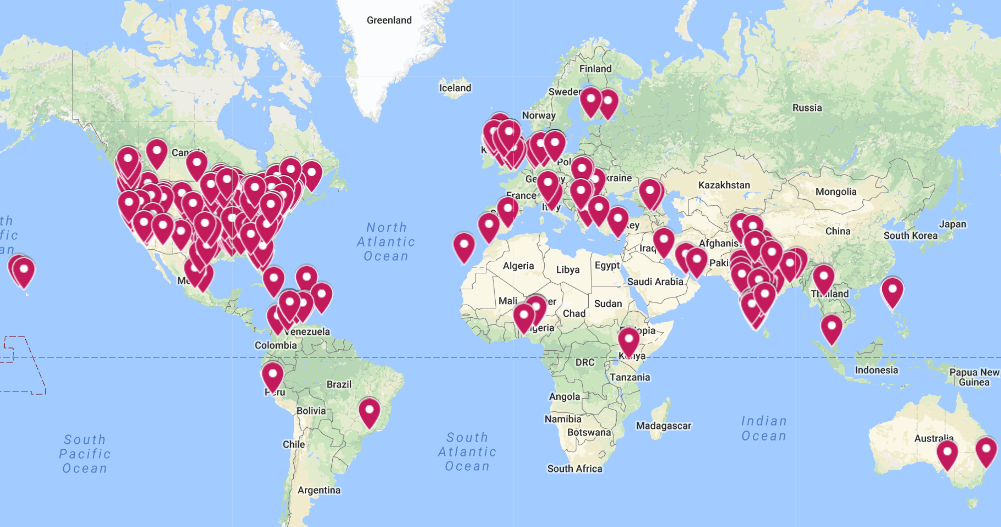
\includegraphics[width=.5\textwidth]{figs/lime/map4.png}
	\caption{Geographical distribution of paid AMT users.}
	\label{fig:map}
\end{figure}


During a 7-day study in May 2018, we kept our (replayed) live video feeds alive, and used Amazon Mechanical Turk (AMT) to recruit 548 paid viewers from 35 countries, with USA and India contributing 78\% of the viewers, as shown in Figure~\ref{fig:map}. Overall, we collected 22 GB data corresponding to more than 4,000 minutes of video viewing. Many paid viewers watched our feeds for more than 4 minutes.  To prevent bias toward viewers with long viewing time, our analysis focuses on only the first 4 minutes per viewer.
During the study, no personally identifiable information was collected.


\section{Understanding Commercial 360\degree{} Live Video Streaming in the Wild}
We now characterize the data collected in \S\ref{sec:lime_data_collection} to reveal the landscape of the performance of today’s popular live 360° video
streaming services.

\subsection{Basic viewer-side QoE metrics}
It is known that three key factors affect the QoE of regular video streaming (both live and on-demand): video quality, stall duration, and quality changes~\cite{yin2015control,huang2015buffer,mao2017neural,dimopoulos2015identifying}. These metrics are also important to panoramic live video streaming so we quantitatively measure them using the AMT dataset. We find that our three videos yield very similar distributions on all metrics. Thus, we present their aggregated results henceforth.

\begin{figure*}[t]
	\centering
	\begin{minipage}{.4\textwidth}
		\centering
		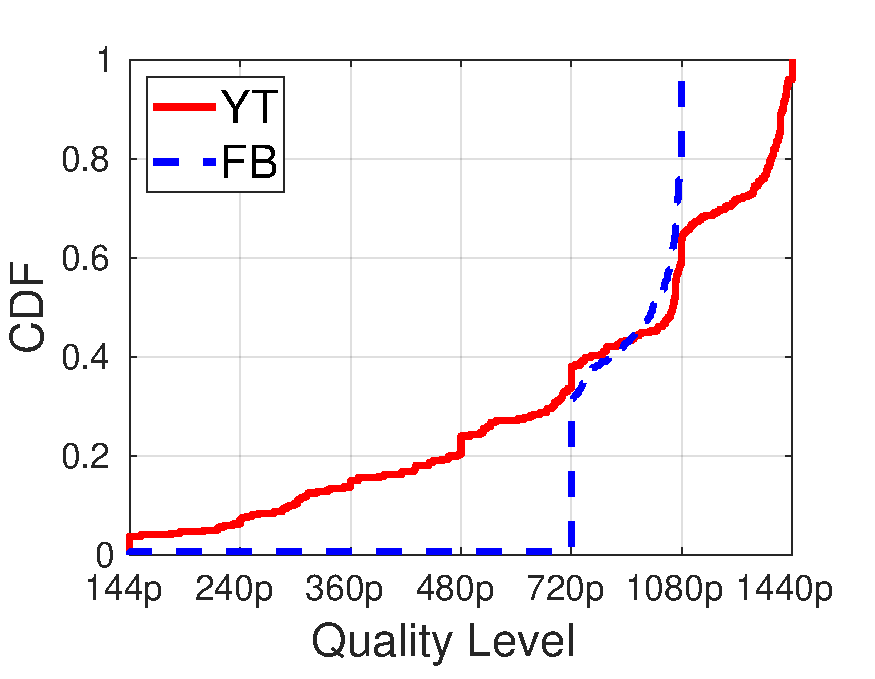
\includegraphics[width=\linewidth]{figs/lime/average_quality.pdf} \vspace{-.25in}
		\caption{\small Average streaming quality across all sessions.}
		\label{fig:average_quality}
	\end{minipage}
	\begin{minipage}{.4\textwidth}
		\centering
		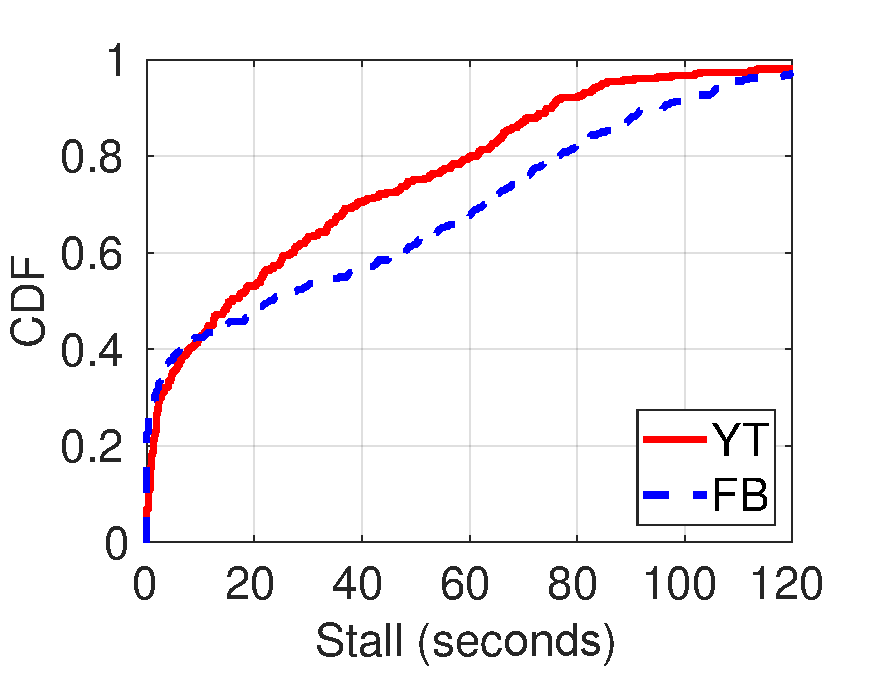
\includegraphics[width=\linewidth]{figs/lime/len_of_stall.pdf} \vspace{-.25in}
		\caption{\small Distributions of per-session stall duration.}
		\label{fig:stall_per_session}
	\end{minipage}
\end{figure*}


\BULLET \textbf{Video Quality.}
Figure~\ref{fig:average_quality} plots the Cumulative Distribution Function (CDF) of the average video quality for YT and FB across all viewing sessions. Recall that each viewing session is a 4-minute 360\degree{} live video content streamed to one paid AMT viewer. As shown in this figure, a key difference between YT and FB is that the average quality for most FB viewers is either 720p or 1080p, which are the only two quality levels provided by FB; in contrast, YT supports 7 quality levels ranging from 144p to 1440p, providing more flexibility as we will discuss shortly.
%a wide range of
%Despite this difference, the median video quality is similar: 4.9 for YT and 4.8 for FB (we use the following quality mapping throughout this paper: 0=144p, 1=240p, 2=360p, 3=480p, 4=720p, 5=1080p, 6=1440p).
Overall, the live 360\degree{} videos' quality is not high, with 34\% (35\%) of YT (FB) sessions having an average quality no higher than 720p.
%
It is important to note that the above qualities refer to the qualities of panoramic frames. Since a viewer perceives only a small portion of the panoramic scene (about 15\% as measured), the actual \emph{perceived} quality is much lower, \eg 15\% of the 720p resolution is between 240p and 360p.

\BULLET \textbf{Stall.} Figure~\ref{fig:stall_per_session} plots the CDFs of the stall duration per session. About 36\% (39\%) of YT (FB) sessions experience less than 5 seconds stalls. However, many users experience very long stalls: 47\% (52\%) of YT (FB) sessions stall for at least 20 seconds (\ie 5 seconds per minute). FB is afflicted by longer stalls than YT, despite their viewing  sessions characterized by similar throughput distributions. Given this, we are leaning towards attributing YT's shorter stall duration to its wider range of quality levels, which allow YT players to flexibly select (lower) streaming bitrates.

We also investigate how stalls are distributed within a session. We find that the vast majority of stall events, which are separated using an inter-stall time of at least 1 second, are fairly short: for YT (FB), the median of their durations are 0.7 (1.0) second.  Note that changing the threshold of inter-stall time to 0.5s or 1.5s yields similar results. 
%
Meanwhile, the number of stall events is large. Figure~\ref{fig:stall_num} plots the CDFs of the number of stall events per session, with the median measured to be 18 (17) for YT (FB), respectively. Compared to fewer long stall events, having more short stall events may bring even worse QoE (\eg motion sickness in VR)~\cite{duanmu2017qoe, moorthy2012qoe, qi06qoe}. %in particular in the VR context. \feng{[[Any paper to cite?]]}

\begin{figure*}[t]
	\centering
	\begin{minipage}{.4\textwidth}
		\centering
		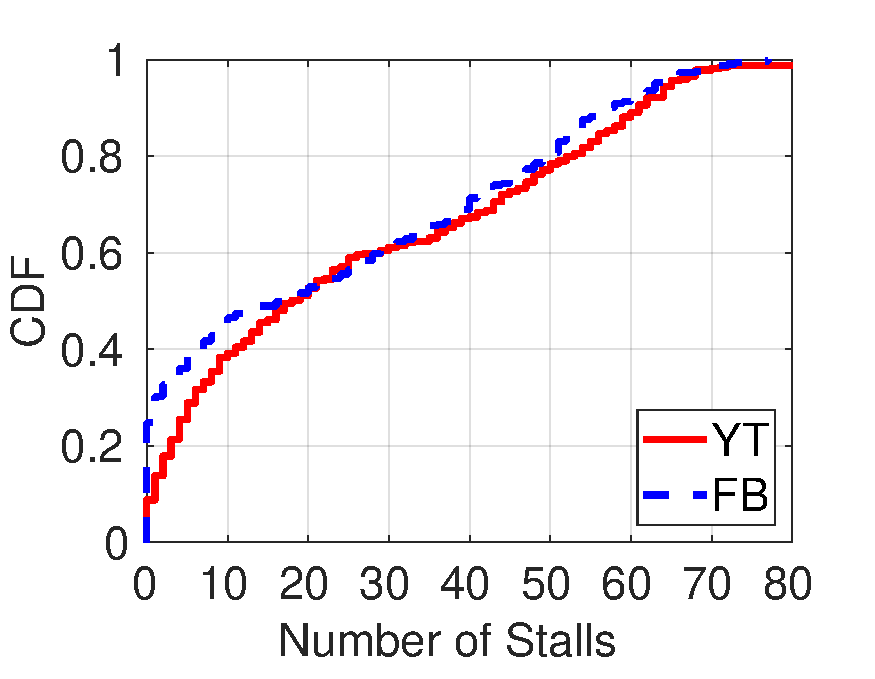
\includegraphics[width=\linewidth]{figs/lime/num_of_stalls.pdf} \vspace{-.25in}
		\caption{\small Distributions of per-session number of stalls.}
		\label{fig:stall_num}
	\end{minipage}
	\begin{minipage}{.4\textwidth}
		\centering
		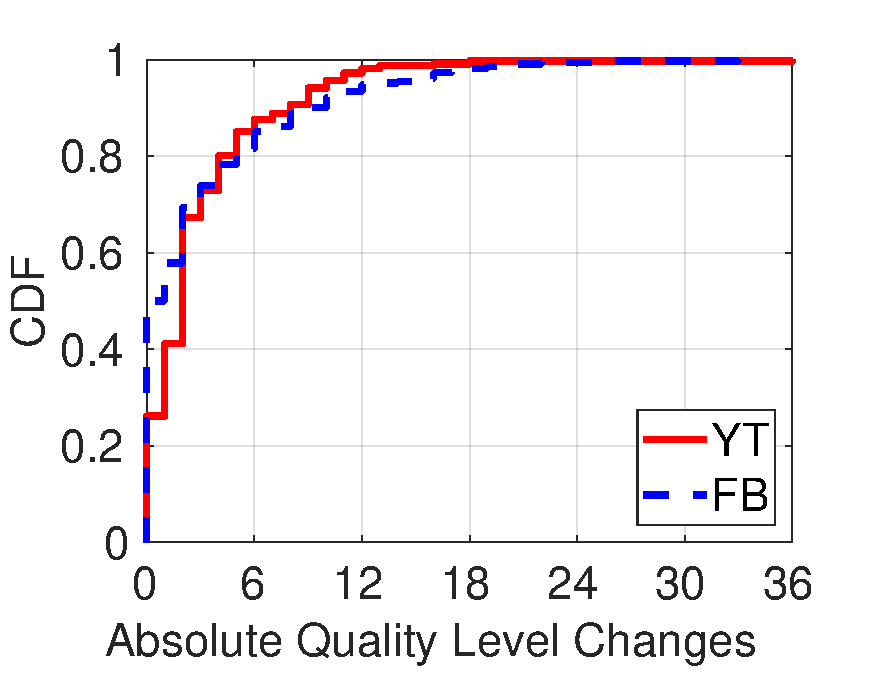
\includegraphics[width=\linewidth]{figs/lime/quality_change.pdf} \vspace{-.25in}
		\caption{\small Distributions of per-session quality level changes.}
		\label{fig:quality_change}
	\end{minipage}
\end{figure*}


%\mvnote{All this need more attention on the bottleneck introduced by the client as discussed.}
Since the stall duration shown in Figure~\ref{fig:stall_per_session} appears to be much higher than those measured by a previous study on Periscope~\cite{siekkinen16}, we attempt to find out the reason. Recall that live video streaming consists of four phases: upload, server-side re-encoding, download, and client-side rendering/playback.
For upload, we ensure high bandwidth between our broadcaster and the streaming servers.
For download, surprisingly, we observe very little correlation between
the per-session stall duration and its network throughput or throughput variation
(Pearson correlation coefficient $<$ 0.1). In fact, many viewers have very high network throughput but still experience high stalls (recall that YouTube can reduce its quality to as low as 144p). For example, one-third of the top 30\% YT sessions in terms of the stall duration are characterized by an average throughput ranked in the top 30\% of the sessions.
%For example, for the top 30\% YT sessions experiencing highest stall durations, 32\% have their average HTTP response throughput ranked at top 30\%.

The above observation makes us believe that for live 360\degree{} video streaming, the performance bottleneck is caused by either the server processing (real-time video re-encoding and possibly projection transformation) or client-side computation/rendering.
%
In particular, we are able to verify that the \emph{client-side overhead} can cause frequent stalls:
when testing on a 2013 MacBook Pro, we observe the CPU utilization of 360\degree{} live streaming can reach up to 80\%, about 60\% higher than non-360\degree{} live streaming. When the CPU is saturated, the live streaming can oftentimes stall.

%which needs to perform real-time video re-encoding and (possibly for 360\DEG videos) projection transformation, which incur high overheads.

\BULLET \textbf{Quality Changes.} Figure~\ref{fig:quality_change} plots the CDFs of the total number of quality level changes per session. When a quality level change occurs, it is counted as $\Delta L = |L_\text{before} - L_\text{after}|$ where $L_\text{before}$ and $L_\text{after}$ are the quality levels before and after the change, respectively. Possible levels are \{0,1,...,6\} for YT and \{4,5\} for FB\footnote{We use the following quality mappings throughout this paper: 0=144p, 1=240p, 2=360p, 3=480p, 4=720p, 5=1080p, 6=1440p.}. We then sum up all $\Delta L$ to get the total quality level changes per session.
%
For most sessions, we did not observe significant quality changes: the median of $\sum\Delta L$ is only 2 and 1 for YT and FB, respectively.
%This is likely attributed to conservative rate adaptation schemes for live streaming that under-utilize the available bandwidth (see \S\ref{sec:xx}).
Nevertheless, we do find about 6\% (10\%) for YT (FB) of sessions with $\sum\Delta L \ge 10$, attributed to the highly variable bandwidth as confirmed from our measured network throughput.



\subsection{Broadcaster-to-viewer (B2V) Latency}
\label{sec:b2v}

\begin{figure}[t]
	\centering
	\centering
	\small
	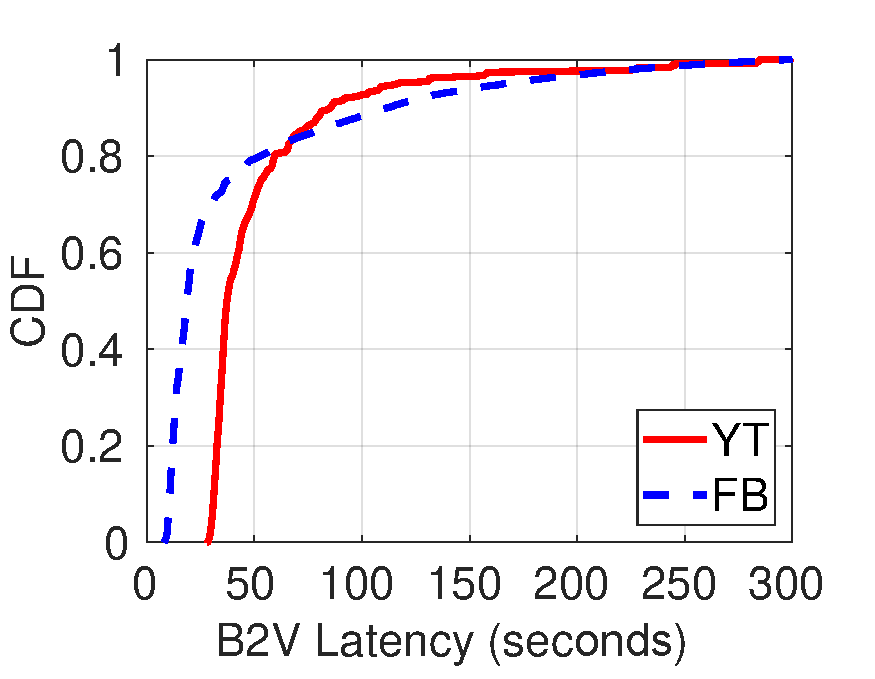
\includegraphics[width=0.4\textwidth]{figs/lime/e2e_latency.pdf}
	\caption{B2V latency of samples across all sessions. In each session, B2V latency is measured every 2 seconds.}
	\label{fig:e2e_latency}
\end{figure}

We apply the method introduced in~\S\ref{sec:b2v_overview} to measure the B2V latency for the AMT viewers, with the results shown in Figure~\ref{fig:e2e_latency}. %We show the results in Figure~\ref{fig:e2e_latency}.
%
We make three observations.
%
First, most sessions have consistent B2V latencies, around 18.7 seconds for FB and 37.1 seconds for YT (median values). Overall, the observed B2V latency is much higher compared to previous measurement on Periscope~\cite{wang16}, which uses push-based RTMP on a subset of users to provide an ultra-low B2V latency (less than 2 seconds).
%\feng{[[Xing: a quick experiment to compare B2V latency between 360 and non-360 live?]]}
%
Second, both platforms exhibit long tails of up to 4.8 minutes for FB and 5.1 minutes for YT. Such high latency inevitably affects viewers' experience.
Although it is difficult to reverse engineer the precise algorithm, we find that throughput appears to be a factor that affects the B2V latency. For example, YT exhibits a negative correlation (Pearson correlation coefficient of -0.4) between the B2V latency and throughput.
%
Third, we also notice that FB exhibits lower B2V latency than YT.
%This can be partly explained by several
This can be explained by several potential reasons.
%
One is that compared to YT, FB has a shorter chunk duration (1 vs 5 seconds) that leads to a lower chunking delay~\cite{wang16}. FB also has a lower polling delay allowing the viewer to update the chunk list more quickly. In addition, recall that a FB server only re-encodes the input video into 2 quality levels while a YT server needs to process 7 quality levels up to 1440p. Such a higher re-encoding overhead may also contribute additional latency.


\section{Adaptiveness in 360\degree{} Live Video Streaming}

We complement our crowd-sourced study with controlled
experiments to shed light on bringing adaptiveness to both
the viewers and the broadcaster. These are the key features
missing from today’s 360\degree{} live video streaming systems. The contribution here
is to quantitatively study its benefits using commercial systems,
realistic live 360\degree{} video content, and real users’ viewing trajectory
traces. In addition, we also identify several inefficiencies in production
360\degree{} live video streaming systems that diminish the benefits of
viewport adaptiveness. We conduct all controlled experiments over
\lime by replacing crowd-sourced viewers with in-lab players. The preliminary results will be discussed in the proposal presentation.


%\chapter{\emph{Improving the Quality of Experience}: Engineering High Quality Untethered Multi-user VR for Commodity Mobile Devices} \label{chap:vr}



\section{Introduction}
Virtual Reality (VR) has registered numerous applications. In
this chapter, we focus on multi-user VR where multiple users
jointly participate in exploring a VR scene. This enables
many applications that single-user VR cannot support such as
team training, social VR, group therapy, collaborative product
design, and multi-user gaming.

We envision the following use case with more than 10 collocated users in a VR room. To start multi-user VR, each user simply launches the app on her smartphone and plugs the phone into a VR headset (\eg a \$50 Samsung Gear VR~\cite{samsung-gear-vr} or even a \$10 Google Cardboard~\cite{google-cardboard} with a \$6 VR controller~\cite{vr-controller}).
These mobile devices fetch the VR content from an off-the-shelf server based on the users' real-time motion. The devices and the server communicate wirelessly over a single WiFi access point (AP). The users can enjoy the high-quality VR content as if it is rendered by a desktop PC with a powerful GPU. Meanwhile, each user can see and possibly interact with other users in the virtual world.

My work therefore aims at realizing the above ambitious use case. We design \firefly, a novel multi-user VR system for mobile devices. The  goals of \firefly are the following.
First, \firefly works with affordable, commercial off-the-shelf (COTS) mobile devices, server, and AP. This helps reduce the deployment cost and facilitate the ``bring-your-own-device'' (BYOD) policies that many enterprises adopt today~\cite{byodref}.
Second, \firefly employs untethered, wireless VR to overcome the inconvenience and trip hazards incurred by wired cables~\cite{triphazard}. This is important for multi-user VR where multiple users' cables may easily get intertwined.
Third, \firefly offers high content quality, low ``motion-to-photon'' (M2P) latency, and high frame rate. An M2P higher than 16ms may cause nausea to VR users~\cite{motionsickness}. We target Quad HD (1440p) resolution, 60 frames per second (FPS) that can provide a good experience even for fast-paced VR gaming -- the most demanding VR task~\cite{vr_gaming}.
Fourth, \firefly aims at supporting $\sim$15 users who can form a sizeable group of, for example, co-workers, students, and patients. To the best of our knowledge, no existing system can achieve this using a single commodity server and WiFi AP. 
Fifth, \firefly allows complex VR scenes with both background and dynamic foreground objects, such as other users' avatars that users can interact with.

The above goals pose tremendous challenges. The CPU/GPU power of a smartphone is at least one order of magnitude lower than its desktop counterpart~\cite{satyanarayanan2019computing}, not to mention the energy/heat constraints;
the heterogeneity of their computational capabilities should also to be taken into consideration;
the bandwidth offered by a single AP is limited for multiple users;
another key challenge is multi-user scalability, which calls for strategic decisions of splitting the client-server workload,
as well as scalable approaches for rendering and distributing the content.
To address the above challenges, \firefly makes a series of judicious design decisions as follows.

\BULLET \firefly performs one-time, offline content preparation by enumerating, pre-rendering, and storing
the views at all positions reachable in a virtual scene. At runtime, given a user's position and viewing direction, the server directly retrieves the stored high-quality content and delivers it to the user. This completely eliminates the online rendering overhead.
Prior work~\cite{boos2016flashback} applies offline rendering to a single mobile device for local VR scenes, while \firefly further extends this concept to networked multi-user VR where offline rendering is found to be an indispensable mechanism ensuring scalability.

\BULLET To reduce the network bandwidth consumption, \firefly takes a viewport-adaptive approach: each user only requests for the content that the user is about to perceive based on motion prediction.
We conduct a thorough analysis of 25 human users' motion traces collected from an IRB-approved user trial.
The results shed light on developing a lightweight yet effective motion prediction approach for \firefly.
%In the literature, several studies~\cite{fan2017fixation,hou2018predictive,bao2016shooting} have examined 360\degree{} video viewers' viewing patterns that only involve rotational movement (yaw and pitch). Our study instead investigates generic VR users' motion that consists of both the rotational and translational viewport movement as well as their interplay (\S\ref{sec:??}).% move this to related work

\BULLET \firefly supports \emph{Adaptive Quality Control (AQC)}, which determines the content quality of each user based on the total network bandwidth, the bandwidth available to each user, and the amount of to-be-delivered content.
AQC essentially extends traditional video bitrate adaptation~\cite{jiang2012improving,huang2014buffer,yin2015control,mao2017neural}:
from handling a single client to multiple clients,
from dealing with regular videos to immersive VR content, and
from being invoked at the second level to the millisecond level to adapt to users' motion.
These differences require AQC to be effective, lightweight, fair, and scalable.

\BULLET \firefly handles dynamic foreground objects in a scalable and adaptive manner.
Specifically, objects' 3D models are distributed to the clients offline.
They are then rendered locally by the client. This eliminates the uncertainty caused by the network as well as the potential resource competition from other users compared to a server-side approach.
To prevent too many objects appearing in the viewport from slowing down client-side rendering, \firefly supports adaptively reducing the objects' fidelity to maintain a high FPS.

We are currently working on the full implementation of \firefly system, in the following part of this section we will discuss the design of \firefly, highlight preliminary results, and point out future works. 

\section{Firefly Overview}

\firefly server exhaustively enumerates all possible views at all positions, renders them at a high quality, encodes them into video frames, and saves the frames in the storage.
%
At runtime, the server simply retrieves and transmits the pre-encoded frames based on each user's position and viewport. In this way, the rendering/encoding overhead at runtime is completely eliminated, so the server can easily scale to tens or even hundreds of simultaneous users. These benefits come at the cost of high storage usage, which is largely not an issue given the cheap storage today.
%
Figure~\ref{fig:system_design} plots the overall architecture. As shown, \firefly consists of a content server and multiple commodity mobile devices. %such as a VR headset with a smartphone plugged in.
They are wirelessly connected through a WiFi access point (AP). This setup can be easily realized in enterprise or home environments at a very low cost.
%
Note that prior work~\cite{boos2016flashback} applies offline rendering to a single mobile device for local VR scenes, while \firefly further extends this concept to networked multi-user VR where offline rendering is found to be an indispensable mechanism ensuring the scalability.

\begin{figure}[t]
	\centering
	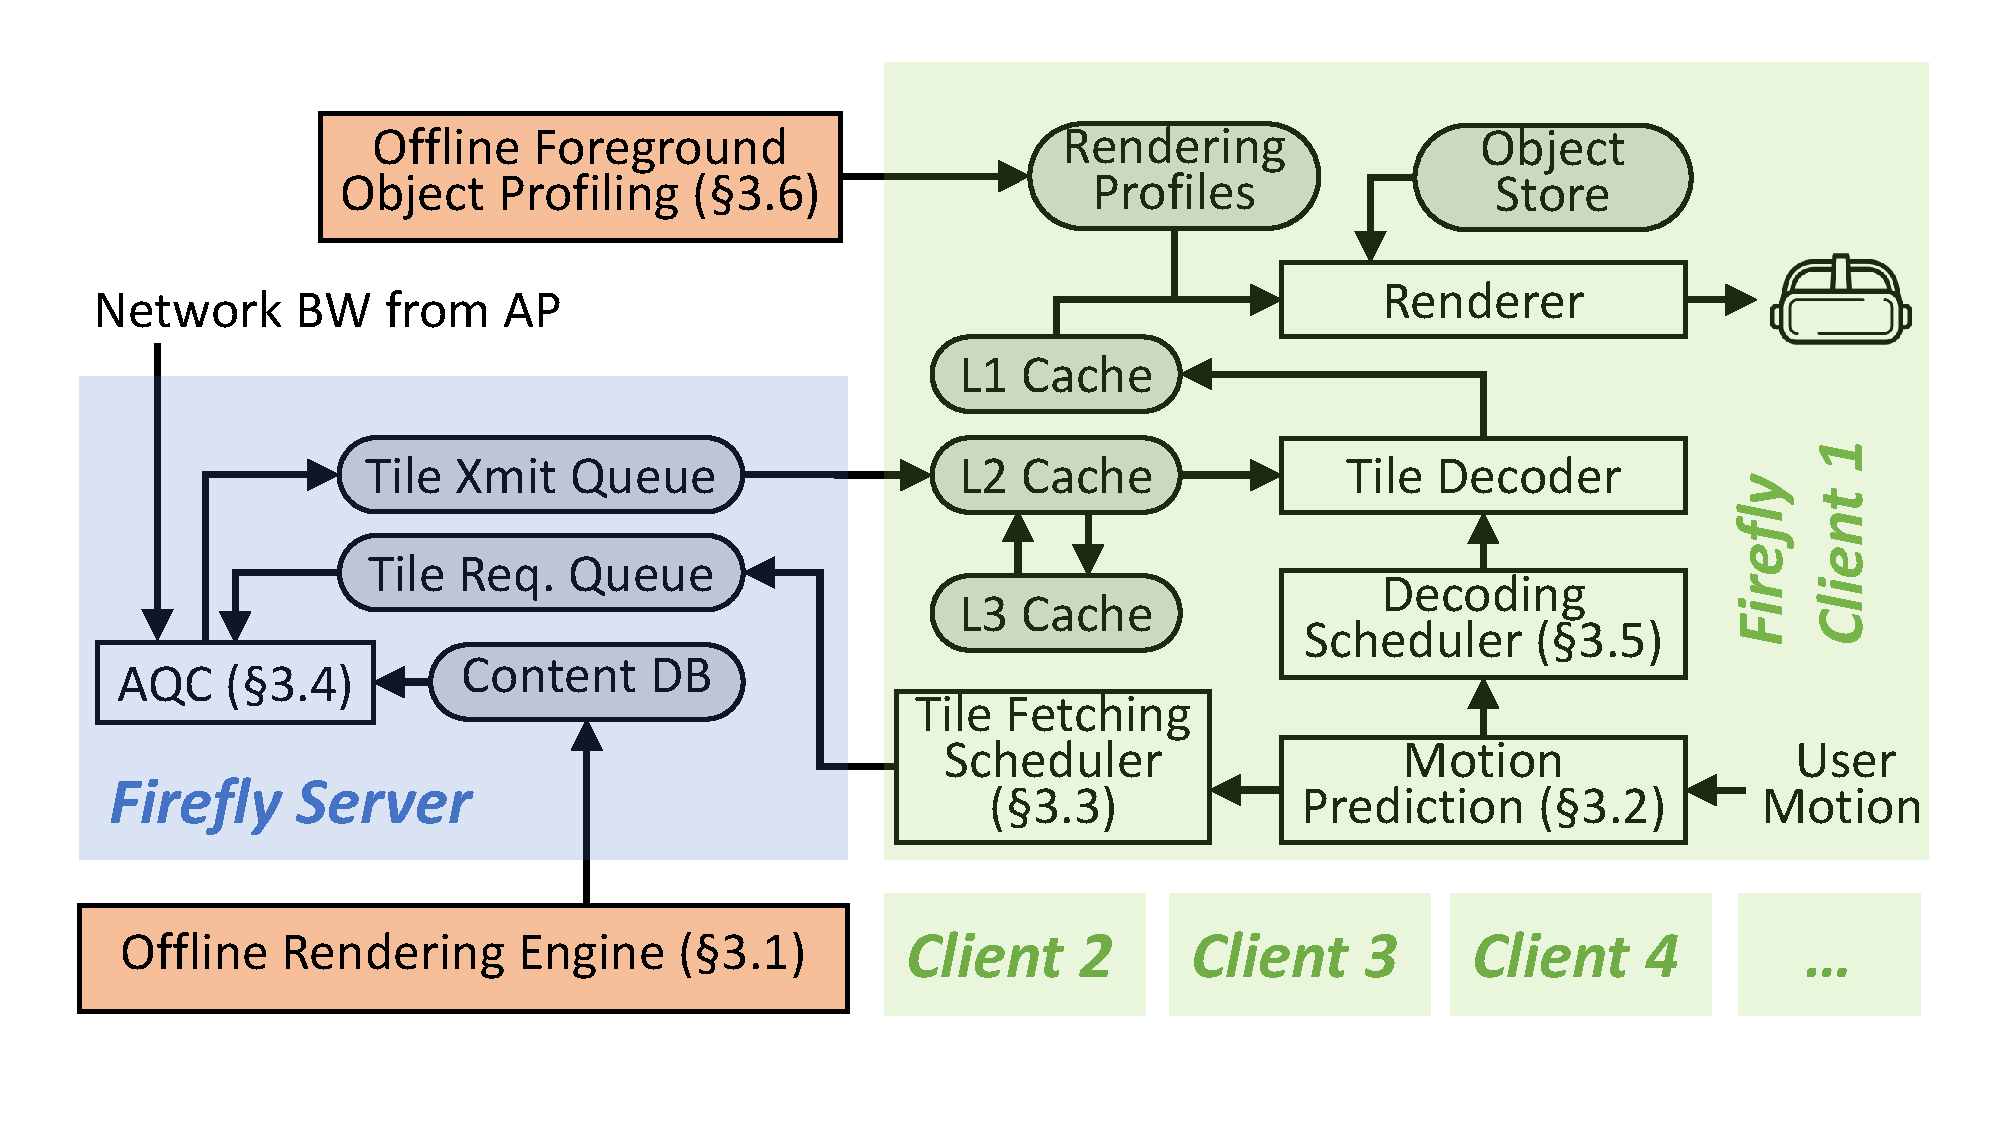
\includegraphics[width=.8\textwidth]{figs/firefly/arch.pdf}
	\caption{The \firefly system architecture.}
	\label{fig:system_design}
	\vspace{-.2in}
\end{figure}

The server consists of a content database that stores rendered/encoded content indexed by a user's position and viewing direction. The database is built by the Offline Rendering Engine that performs the aforementioned exhaustive content generation.
%
Another critical component is the AQC module that is introduced to scale the system and to handle the wireless bandwidth fluctuation. It determines in real-time the content quality for each user.
%
Designing AQC is challenging due to multiple requirements including boosting users' QoE, maintaining good performance, ensuring scalability, and achieving fairness.

On the client side, there are two high-level design choices on the content fetching strategy for background frames.
%on the client side.
First, the client can prefetch all surrounding frames at every new virtual position~\cite{lai2019furion}.
%similar to Furion~\cite{lai2019furion} scheme.
However, this technique may consume high bandwidth with a considerable amount of wasted traffic (\ie the fetched content is not viewed by the user), making it infeasible for multi-user VR.
%
Second, to reduce the bandwidth footprint, the client can use its historical motion trajectory to predict the future viewport and to
prefetch only the portions that will likely be consumed in the near future. \firefly is the first to incorporate this viewport-adaptative approach into generic VR using robust motion prediction (\S\ref{sec:motion_prediction}).
%The client also uses an efficient hierarchical cache management (\S\ref{sec:cache}).
The client also efficiently manages its local cache and handles foreground dynamic objects in an adaptive and scalable manner.

\begin{figure*}[t]
	\centering
	\begin{minipage}{.4\textwidth}
		\centering
		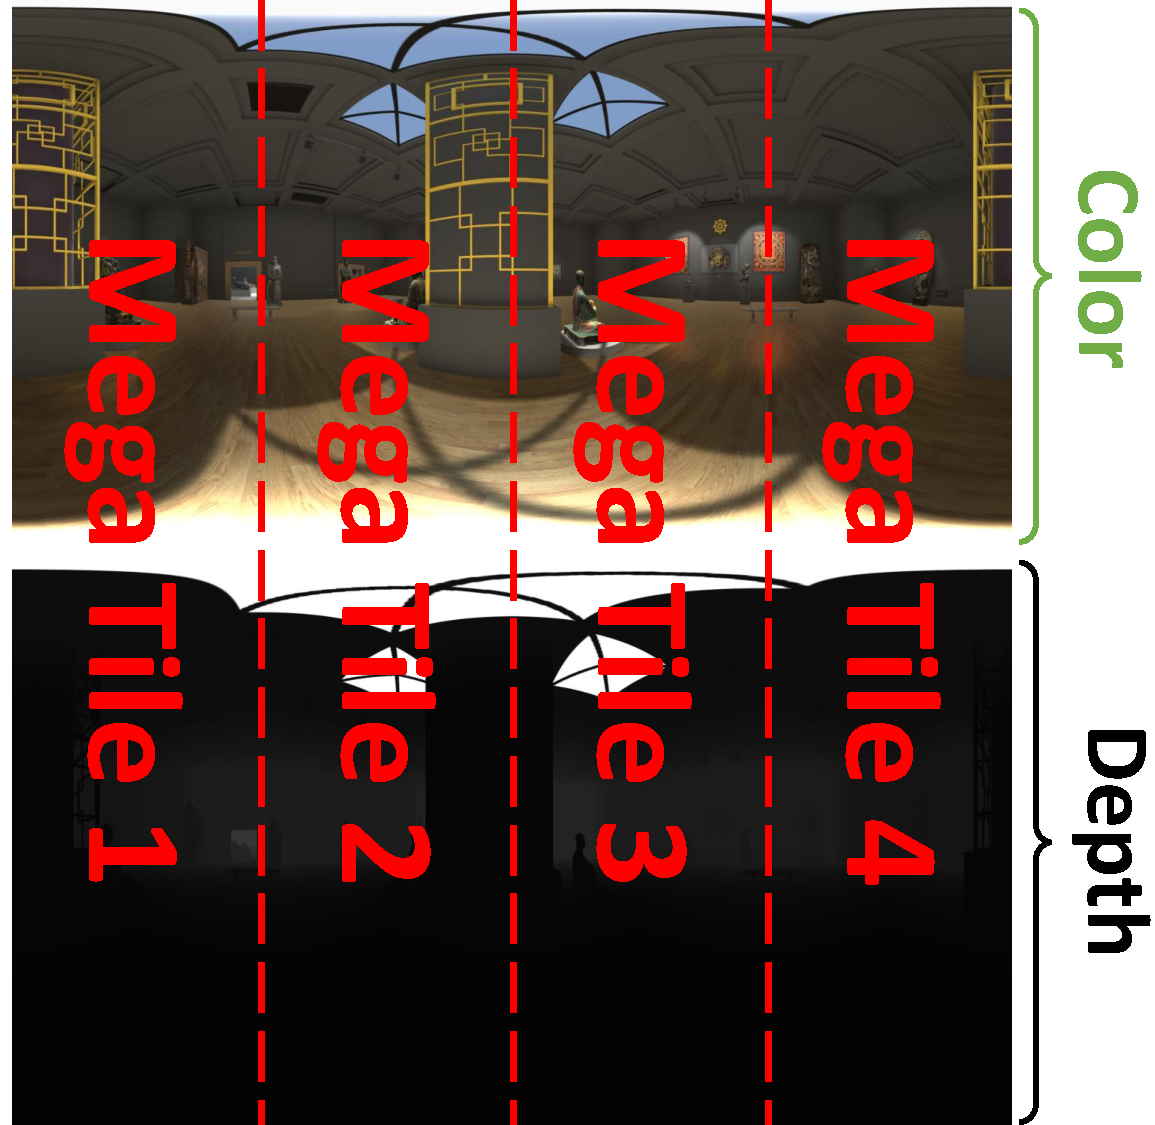
\includegraphics[width=\linewidth]{figs/firefly/MT.pdf}
		\vspace{-.1in}
		\caption{\small Mega frame.}
		\label{fig:mf}
	\end{minipage}
	\begin{minipage}{.5\textwidth}
		\centering
		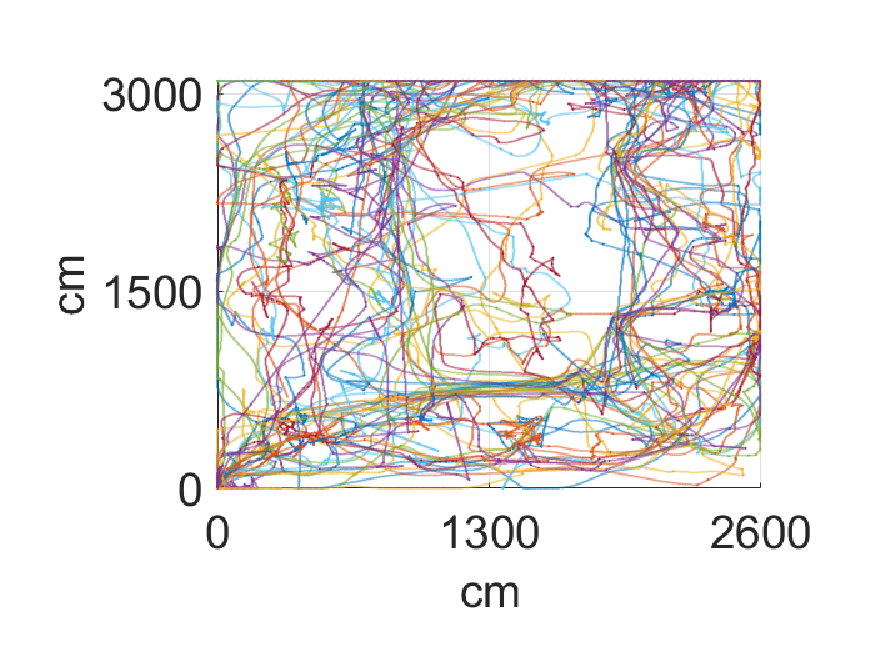
\includegraphics[width=\linewidth]{figs/firefly/office_trajectory.pdf} \vspace{-.25in}
		\caption{\small Users' translational trajectories (the Office scene).}
		\label{fig:office_trajectory}
	\end{minipage}
\end{figure*}

\subsection{Offline rendering engine}
The offline rendering engine produces the content database.
%The detailed content generation process is as follows.
%
The whole VR world is discretized into grids. At each grid position that the user can reach, the rendering engine renders a \emph{mega frame} that captures the 360\degree{} panoramic view that the user can possibly perceive at a high quality. \firefly uses Equirectangular projection~\cite{equirectangular} to generate the panoramic representation, but other projection algorithms~\cite{pyramid,cubemap,yu2015framework} can also be applied. As shown in Figure~\ref{fig:mf}, besides the color frame (top), a mega frame also includes a panoramic depth map (bottom) where the brightness of each pixel indicates its distance from the user. The depth map will be used to ensure the correct occlusion when overlaying foreground objects such as avatars of other users onto the scene. %In other words, a mega frame captures the panoramic 3D environment at each position.

We next apply the \emph{tiling} technique~\cite{qian2018flare,he2018rubiks} by dividing each mega frame into \emph{mega tiles}. Each tile is independently encoded and can be separately transmitted and decoded.
%
The rationale is that, since the user only sees a portion of the whole panoramic scene at a given time, there is oftentimes no need to fetch the entire mega frame. The mega tiles thus allow users to (pre)fetch the content more adaptively at a finer granularity, to reduce the network bandwidth consumption.
%
The tiling scheme requires the user to predict its viewport, \ie to determine which tiles to fetch based on the observed viewport trajectory.

A decision we need to make is to determine the number of tiles and their layout.
While having more tiles provides more bandwidth saving opportunities, in the meantime it increases the decoding overhead %\xing{we just mentioned it reduces decoding overhead}
and makes compression less efficient.
%The latter is because similar content falling into different tiles has to be separately encoded, incurring redundant data.
After carefully studying the above tradeoffs using real users' viewport trajectory data (\S\ref{sec:motion_prediction}), we decide to vertically segment each mega frame into four mega tiles as shown in Figure~\ref{fig:mf}. We choose vertical segmentation because according to our data collected from 25 users,
users tend to keep their sight vertically centered (\ie looking at the equator) while moving the viewport horizontally.
%
This makes horizontal segmentation at the equator (0\degree{} latitude) inefficient because the vertically centered viewport will always overlap with at least two tiles, \ie one above and the other below the equator.

As described above, at each position, the offline rendering engine renders four tiles capturing the panoramic view and depth. Each tile is then independently encoded into video frames with multiple quality levels.
%
The rendered and encoded tiles are stored in the content database, indexed by the user's grid position, the tile ID (1 to 4), and the quality level.


\section{VR Viewport Movement: Characterization and Prediction}
\label{sec:motion_prediction}

Users' motion makes VR immersive and interactive. In the literature, many studies have investigated users' head \emph{rotational} movement when watching 360\degree{} videos~\cite{fan2017fixation,hou2018predictive,bao2016shooting}. Generic VR differs from 360\degree{} videos in that it further involves \emph{translational} movement.
%
To our knowledge, no prior study has comprehensively investigated VR users' motion patterns and their predictability, which are our focus here.

\begin{figure*}[t]
	\centering
	\begin{minipage}{.45\textwidth}
		\centering
		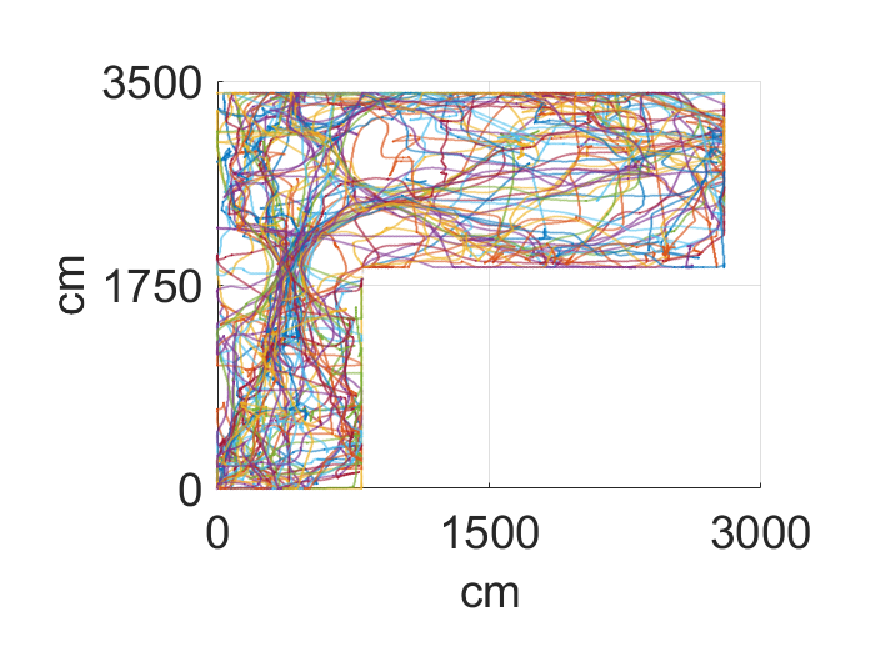
\includegraphics[width=\linewidth]{figs/firefly/museum_trajectory.pdf}
		\caption{\small Users' translational trajectories (the Museum scene).}
		\label{fig:museum_trajectory}
	\end{minipage}
	\begin{minipage}{.45\textwidth}
		\centering
		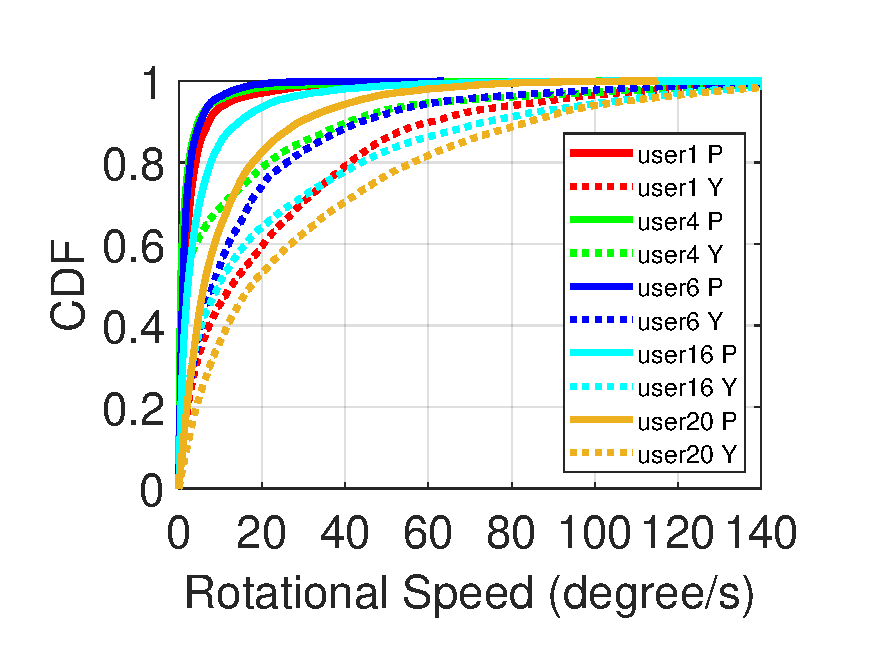
\includegraphics[width=\linewidth]{figs/firefly/angular_velocity.pdf}
		\caption{\small Five users' rotational speed (P=Pitch, Y=Yaw).}
		\label{fig:angular_velocity}
	\end{minipage}
\end{figure*}


\textbf{Collecting Viewport Movement Data from Real Users.} We conduct an IRB-approved user study involving 25 voluntary participants recruited from a large university. Among the 25 users, 9 are female. The users are from 8 departments as undergraduate (16), master (4), and Ph.D. students (5). %12 of them have prior experiences with VR.
During the study, each subject wears an Oculus Rift headset~\cite{rift} connected to a high-end PC. The subject can freely make rotational movement by moving her head as well as perform translational movement using the handheld controller.

We obtain two large VR scenes from the Unity store: Office~\cite{office} (30m$\times$26m) and Museum~\cite{museum} (35m$\times$30m, L-shape). We then develop a custom VR system (different from \firefly) that loads each scene for the users to explore. Our system logs from each user the precise viewport trajectory.
%including the viewpoint position and viewing direction.
%
We let each subject explore each scene in a random order for 5 minutes, with an arbitrarily long break allowed between the two sessions.
%
%After the study, most subjects agreed that the user experience was good, while some told us the VR headset's cable caused a bit inconvenience -- this is exactly why we need untethered VR in particular for multi-user. %Each participant received a \$20 compensation for participating our study.
We will make our dataset publicly available.

\textbf{Motion Trace Characterization.}
We now characterize the unique dataset above
%Leveraging the above unique dataset, we now present measurement results
to reveal VR users' motion dynamics and to provide insights for \firefly's design.
%
To begin with, Figure~\ref{fig:office_trajectory} and~\ref{fig:museum_trajectory} plot the translational movement trajectories of all users, represented by different colors, for the two VR scenes.
%
As shown, in most locations, the users' trajectories are highly heterogeneous.
%Similar observations are made for rotational movement trajectories (figure not shown). In contrast, prior studies have shown that for 360\DEG videos, different users oftentimes exhibit common interested regions in many frames~\cite{xx}. While the content difference may play a role, we think another reason is that compared to 360\DEG videos, generic VR includes more dimensions that increase users' motion diversity.
This finding suggests that the server should not use broadcast or multicast, simply because users typically see different content at a given time.

Fast motion may cause difficulties for viewport prediction. We thus quantify the users' motion speed.
The translational movement speed is fixed at 1m/s (set based on reported experiences from another user study)
when the user presses the controller button.
%
Figure~\ref{fig:angular_velocity} plots the distributions of rotational movement speed, calculated by sliding a 500ms window over the trajectory, across all window positions for five randomly selected users. As shown, the users exhibit different speeds, whose medians range from 1.3\degree{}/s to 18.6\degree{}/s for yaw and from 0.5\degree{}/s to 7.0\degree{}/s for pitch.
%
The median speed across all 25 users is 10.2\degree{}/s and 2.4\degree{}/s for yaw and pitch, respectively. Interestingly, such speeds match those for typical 360\degree{} users~\cite{qian2018flare}, implying
that translational movement does not necessarily slow down the rotational movement.


\begin{figure*}[t]
	\centering
	\begin{minipage}{.25\textwidth}
		\centering
		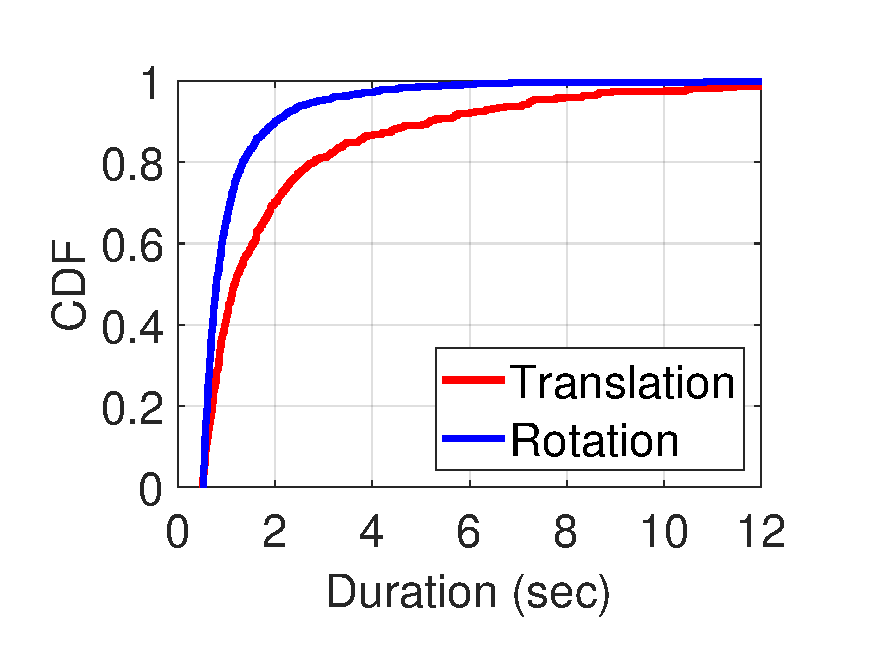
\includegraphics[width=\linewidth]{figs/firefly/per_pause_duration.pdf} \vspace{-.25in}
		\caption{\small SP\\ duration per pause.}
		\label{fig:per_pause_duration}
	\end{minipage}
	\hspace{-.1in}
	\begin{minipage}{.25\textwidth}
		\centering
		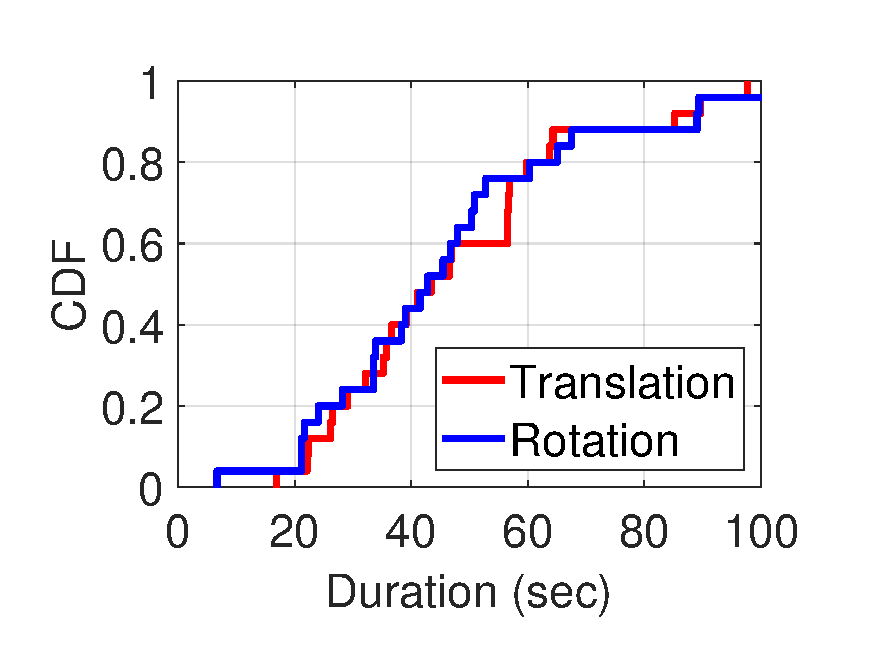
\includegraphics[width=\linewidth]{figs/firefly/total_pause.pdf} \vspace{-.25in}
		\caption{\small Total\\ SP per user.}
		\label{fig:total_pause}
	\end{minipage}
	\hspace{-.1in}
	\begin{minipage}{.25\textwidth}
		\centering
		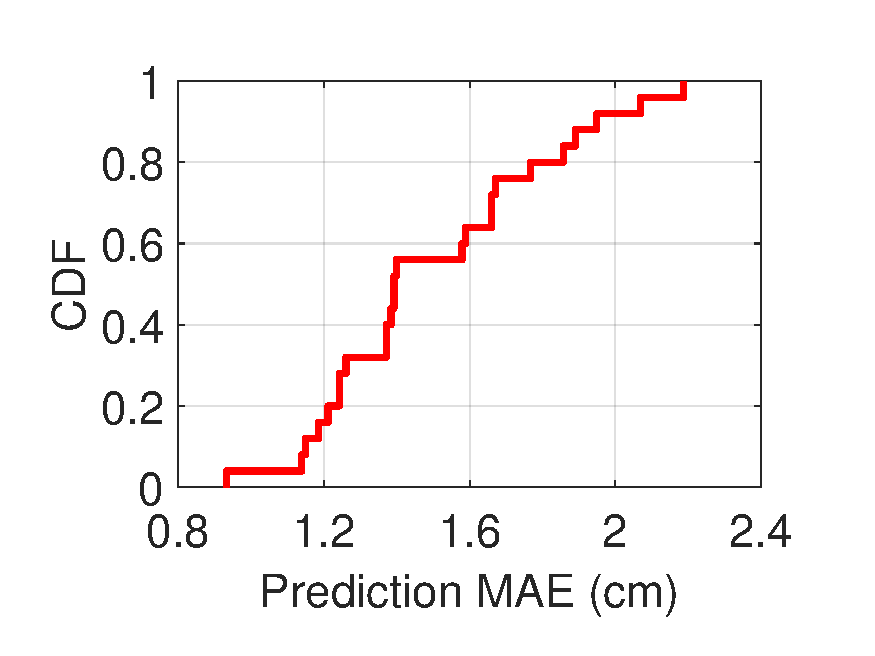
\includegraphics[width=\linewidth]{figs/firefly/translation_mae.pdf} \vspace{-.25in}
		\caption{\small Trans.\\ prediction MAE.}
		\label{fig:translation_mae}
	\end{minipage}
	\hspace{-.1in}
	\begin{minipage}{.25\textwidth}
		\centering
		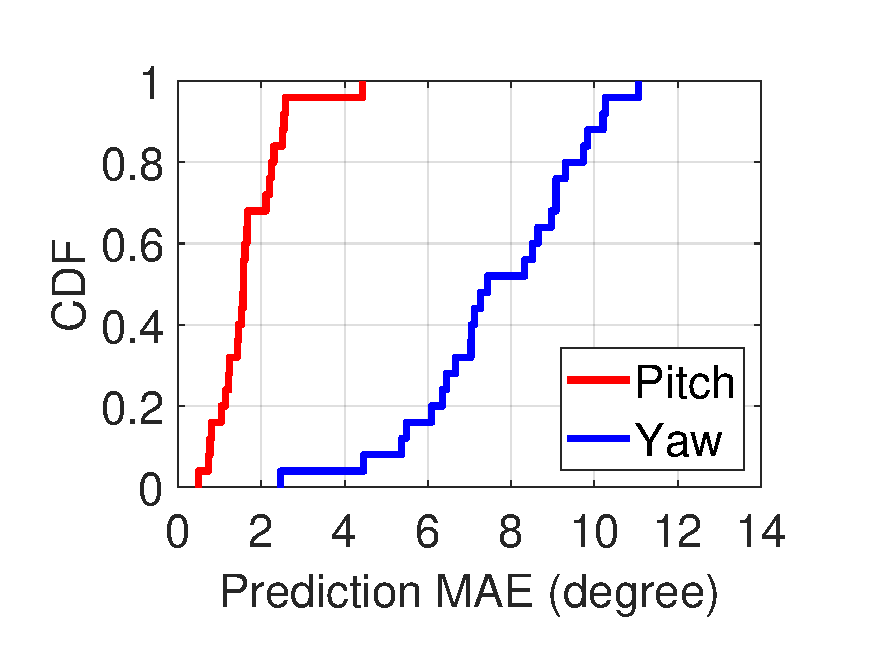
\includegraphics[width=\linewidth]{figs/firefly/rotation_mae.pdf} \vspace{-.25in}
		\caption{\small Rot.\\ prediction MAE.}
		\label{fig:rotation_mae}
	\end{minipage}
	\vspace{-.2in}
\end{figure*}


Another challenging scenario is users' sudden movement after a stationary period. How often do stationary periods (SPs) occur? Figure~\ref{fig:per_pause_duration} plots the distributions of SP duration per pause, which by our definition has to last at least 500ms. %yaw+pitch<2deg 500ms
%
Figure~\ref{fig:total_pause}  plots the total SP duration per user.
As shown, an SP is typically short: 69\% of translational SPs and 89\% of rotational SPs are shorter than 2 seconds. However, Figure~\ref{fig:total_pause} indicates that they occur frequently: within a 5-min VR session, a typical user spends 43 seconds (median) being stationary. Such frequent SPs lead to bursty, non-continuous movement patterns that pose difficulties for viewport prediction.
%
To deal with SPs, we design mechanisms such as conservative tile scheduling and bandwidth reservation (\S\ref{sec:prefetch}).
%
We also find that translational and rotational SPs are not correlated, \ie
a user is typically looking at a fixed direction while moving, or looking around while standing still.
This motivates us to separate the translational and rotational dimensions when performing viewport prediction (see below).

\textbf{Viewport (Motion) Prediction} is required by the tiling scheme.
We make two decisions regarding \firefly's viewport prediction scheme.
%
First, we decide to run it distributively on client devices to make the server scalable.
%
Second, given the above measurement results, we predict each dimension separately (yaw/pitch for rotational movement and X/Y/Z for translational movement), and then combine
them into the final predicted view. We find that this strategy greatly reduces the computational complexity while achieving a decent accuracy -- a desirable tradeoff we want to strike.
%
Regarding the actual algorithm, we continuously train a linear regression (LR) model using the motion trajectory observed within a history window of $H$ milliseconds; we then use this model to predict the future trajectory within a prediction window of $P$ milliseconds before discarding the model. The simple LR model is found to very lightweight yet effective for 360\degree{} videos~\cite{qian2018flare}; here we investigate its effectiveness for generic VR motion prediction. 
%
Ideally, $P$ should be set to the duration of the entire tile processing pipeline (form request being sent to tiles being decoded) plus some safety margin. Guided by this, we set $P$ to 150ms based on empirical profiling. We set $H$ to 50ms based on cross-validating different values of $H$, which is found to not qualitatively impact the prediction accuracy.

Figure~\ref{fig:translation_mae} and~\ref{fig:rotation_mae} plot the prediction results
for translational and rotational movement, respectively, across all users ($H$=50ms, $P$=150ms, the Office scene), with the SPs excluded.
%
The accuracy metric is the mean absolute error (MAE, in distance or degree). %The stationary periods are excluded.
The overall accuracy is high: the median MAE is around 1.4 cm for translational movement, and 1.6\degree{}/7.4\degree{} for vertical (pitch) / horizontal (yaw) rotational movement. The results for the Museum scene are similar.


\section{Future Work}
\subsection{Client-side tile fetching scheduling}
\label{sec:prefetch}
Based on the viewport prediction results, the client needs to judiciously determine which (mega) tiles
to (pre)fetch and in which order. Meanwhile, Due to users’ randomness,
viewport prediction errors are inevitable. \firefly therefore needs to apply a client-side tile (pre)fetching mechanism which also tolerates viewport prediction errors by reserving bandwidth conservatively. The design and implementation of such scheduling algorithm will be my next step.

\subsection{Adaptive quality control (AQC)}
\label{sec:aqc}
AQC takes as input the lists of tiles requested by the users,
and outputs each user’s appropriate quality level. It runs on
the server that has the global knowledge of all users. An ideal
AQC algorithm has the following features. (1) For each user,
AQC will maximize the quality level while minimizing the
stall (rebuffering); meanwhile, the number of quality switches
should be minimized to provide a smooth user experience.
(2) The selected quality levels should be fair across all the
users; in other words, the quality levels should be largely
proportional to the users’ wireless channel capacities. (3)
AQC needs to execute in a fast-paced manner (ideally at the
per-frame granularity for each user) to adapt to users’ motion.
(4) AQC should scale well for multiple users. The design and implementation of \firefly AQC module algorithm will be part of my future work.
 
\subsection{Handling dynamic foreground objects}
A VR scene may consist of a background view as well as
one or more foreground objects. The background view at
a specific virtual location is static. Due to its large area and
complexity, its rendering typically dominates the workload for
preparing the scene. In contrast, foreground objects are more
dynamic and less complex than a background scene. Their
examples include moving objects (\emph{e.g.}, other users’ avatars)
and interactive objects (\emph{e.g.}, a virtual control panel). Despite
being less complex than the background view, due to their
dynamic and interactive nature, failure to render foreground 
objects in time may also cause considerable QoE degradation. My plan on this is to design and implement an adaptive foreground objects rendering scheme. Specifically, objects’ 3D models will be distributed
to the clients offline. They are then rendered locally
by the client. This eliminates the uncertainty caused by the
network as well as the potential resource competition from
other users compared to a server-side approach. To prevent too
many objects appearing in the viewport from slowing down
client-side rendering, \firefly should support adaptively reducing the
objects’ fidelity to maintain a high FPS


%\chapter{\emph{Optimizing the Energy Efficiency}: Characterizing Wearable Usage In The Wild} \label{chap:wearable}



\section{Introduction}
\begin{table}[t]
\centering
\footnotesize
\begin{tabular}{c|l}
\multicolumn{1}{c|}{Topic}  & \multicolumn{1}{c}{Key Results} \\
\hline
 Device states & Dozing dominates the usage (50.6\%); wake-up accounts for 2\% of usage period; \\& wake-up sessions are short but frequent (72 per day on average) with various root \\& causes  such as ``flick and look'' and push notifications. \\
\hline
 Push notifications  & Push notifications are used by 200+ apps, dominated by IM/emails, and exhibiting \\& bursty arrival patterns.  \\
\hline
 Smartwatch apps     & A wide spectrum of watch apps are observed; their execution is dominated by short \\& background services. \\
\hline
 Power models        & Accurate and comprehensive power models for two popular watches. The models \\& have error rates $<$6\%. \\
\hline
 Energy utilization  & Dozing and wake-up account for 56\% and 27\% of overall energy respectively. At \\& component level, CPU (29\%) and display (30\%) dominate the energy consumption. \\& Network consumes only 3.4\% of the energy. \\
\hline
 Energy optimization & ``What-if'' analysis over real data for improving energy efficiency; impact of state \\& machine on battery drain. \\
\hline
 Network traffic     & Watches are paired with phones during 84\% of the daytime; most flows are small, \\& short, slow, and bursty. \\
\end{tabular}
%\vspace{-.1in}
\caption{\footnotesize Key results and findings of smartwatch study.}
%\vspace{-.1in}
\label{tab:toc}
\end{table}

Smartwatch carries numerous ``simplified'' mobile applications and it has become one of the most popular wearable computers on the market, it offers great convenience to end users through a wide range of
features such as receiving push notifications, issuing voice control,
monitoring fitness, and interacting with 3rd-party apps. Despite
its popularity, smartwatches are still relatively new to the
commercial mobile device family, and the research community
lacks a thorough understanding of the smartwatch ecosystem. 

Smartwatch is operating under tight energy budget, typically its battery capacity are 3 quarters less than that of a smartphone. The very first step towards optimizing its energy efficiency is to systematically understand its usage in the wild. We bridge the gap by conducting an IRB-approved crowd-sourced measurement study of smartwatches involving 27 users. We first demonstrate it is feasible to build
a self-contained and comprehensive measurement data collector
on today’s off-the-shelf Android smartwatches. The collector
transparently collects a wide range of usage data, network traffic,
and system events in realistic usage scenarios, with very low
runtime and energy overhead incurred. We then provide each
of the 27 users with a state-of-the-art smartwatch instrumented with
the data collector. Using a 106-day dataset collected from our participants, we conduct an in-depth characterization of three key
aspects of smartwatch usage “in the wild”: usage patterns, energy
consumption, and network traffic characteristics. This is to our
knowledge the most comprehensive and in-depth crowd-sourced
study of smartwatches. Our key measurement results consist of
the following.

\BULLET We characterize the smartwatch usage patterns. An Android
watch can stay in one of the four states with diverse power
characteristics: fully awake, dozing (with dimmed watch face
display and restricted system activity), sleeping (screen further
turned off), and charging. We find that smartwatch’s wake-up
period accounts for only 2\% of the overall usage period among
the four states. The wake-up sessions are not only short, but
also frequent (72 times per day on average). We then analyze
their triggering factors, which help us identify key usage scenarios
of a watch: short ``flick and look'' sessions (the most common
interaction type that the OS needs to be optimized for), push
notifications, longer interaction sessions, and unintended wake-up.

\BULLET A key usage scenario of smartwatches is to receive push
notifications. In our dataset, more than 200 apps send push
notifications to the watch through either the OS-provided Android
Wear service or custom data channels between phone-side and
watch-side apps. Push notifications are dominated by instant
messaging and emails. Despite a potential lack of long-term
predictability, push notifications’ arrival exhibits a strong bursty
pattern, with a median inter-arrival time of only 49 seconds. Also
there is room for the OS to improve push notification delivery, by
strategically determining whether to push and how to push.

\BULLET We also investigate how smartwatch applications (apps) behave.
We find smartwatch app execution is dominated by short but
frequent background services, whose total duration is more than
50 times longer than that of full-screen activities, which users
seldom launch due to a watch’s small form factor making fullfledged
interaction challenging. The services, together with the
OS infrastructures (\emph{e.g.}, the push notification and card management
subsystems) should therefore be the optimization focus for OS and
app developers.

\BULLET We derive comprehensive and accurate power models for two
popular Android smartwatches. We then apply the power
models to the user study data to quantify the energy consumption
of smartwatches in the wild. We made several interesting
observations. More than half of the smartwatch energy is consumed
by the dozing state (56\%) due to its long duration. Meanwhile, the
awake state also plays an important role in energy consumption
(27\%) despite its very short usage duration (2\%). Due to the
big power consumption gap between awake and dozing/sleeping,
a small increase of the wake-up duration will be ``amplified'' from
the battery draining perspective, thus shortening the standby time of
the watch. The top-2 energy-hungry components on smartwatches
are the same as those on smartphones: CPU and display. Despite
smartwatches’ small screen sizes, display still contributes to 30.2\%
of the overall energy. CPU accounts for 29.3\% of the overall
smartwatch energy. Network interfaces, however, consume a
very small fraction of energy on smartwatches without a cellular
interface.

\BULLET We investigate how to make smartwatches more energy-efficient
using combined approaches of trace-driven ``what-if'' analysis
and controlled in-lab experiments. Our results suggest that
the energy efficiency can be further improved through a wide
range of optimization strategies such as optimizing the display,
bundling delay-tolerant push notifications, and dynamically
configuring CPU’s online cores and frequencies. Also the watch’s
state machine and its associated timers affect the
energy consumption and need to be strategically determined, as
demonstrated by our ``what-if'' analysis. 

Our key measurement findings are listed in Table~\ref{tab:toc}. 
To summarize, the major contributions consist of the following.
\begin{itemize}
	\item We develop a self-contained and lightweight measurement data
	collection system for Android Wear smartwatches, and conduct a
	real deployment on 27 users.
	\item We derive accurate and comprehensive power models for two
	commodity Android Wear watches.
	\item We perform systematic measurements of smartwatches’ usage
	patterns, energy consumption profiles, and network traffic characteristics
	using a 106-day dataset collected from 27 users. Based on
	our findings, we identify key energy inefficiencies in the smartwatch ecosystems
	that can be further improved, and propose recommendations via trace driven ``what-if'' analysis.
\end{itemize}



\section{The Smartwatch User Study}
We launched an IRB-approved user study which is open to students, faculty, and staff members on our campus. We recruited 27
participants from more than 200 applicants.
%
Each user was provided with an LG Urbane watch, a high-end smartwatch as of early 2016 (cost $\sim$\$250 USD). It is equipped with a quad-core Cortex A7 processor, 4GB storage, 512MB memory, Wi-Fi, Bluetooth, and various sensors. The watch runs Android Wear OS 1.3, which is based on Android 5.1.1.

\begin{table}[t]
	\centering
	\footnotesize
	\begin{tabular}{l|l|l}
		\multicolumn{1}{c|}{Collected Data Item}   & \multicolumn{1}{|c}{Method$^*$} & \multicolumn{1}{|c}{Source} \\
		\hline
		Wi-Fi packet trace                       & E    & tcpdump \\ %Event triggered \\
		Bluetooth packet trace                   & E    & BT Snoop Logger\\ %Event triggered \\
		User input events                        & E    & /dev/input/ \\
		Voice control input event                & E    & Android Wear log \\ %Event triggered \\
		Device wakeup/doze/sleep                      & E    & Android Wear log \\
		Device charging                          & E    & Android Wear API \\ %Event triggered \\
		Card post                                & E    & Android Wear API \\
		App activity/service state               & E    & atrace \\  %(create/start/stop/pause/resume)
		%Others (\eg network change)              & E    & (misc.) \\ %Event triggered \\
		%\comment{Battery level}          & P (5mins) \\
		Installed apps list                      & P (1 hour) & /data/app/ \\ %Periodically, every 5 mins \\
		Screenshot                               & P (30 sec) & screencap \\ %Periodically, every 5 mins \\
		CPU utilization                          & P (1 sec)  & /proc/stat \\ %Periodically, every 1s \\
		Screen brightness level                  & P (5 sec)  & Android Wear API \\ %Event triggered \\
		\hline
		\multicolumn{3}{l}{$^*$E = event triggered callback; P (interval) = periodical polling}
	\end{tabular}
	\vspace{-.1in}
	\caption{\footnotesize Types of data collected in the user study.}
	\vspace{-.1in}
	\label{tab:data}
\end{table}

We developed our own, which collects a wide range of data listed in Table~\ref{tab:data} in the background. The data collector was written in Java and native C/C++ with about 6,500 LoC.
%
Note the collector only runs at the watch side (the watch is rooted) and does not require any change on users' smartphones (which are usually not rooted).
The collected data is automatically uploaded to our secure server over Wi-Fi at night when the watch is being charged.
The data collection and upload processes are completely transparent to users.
%
As listed in Table~\ref{tab:data},
most data items are collected using event-triggered callbacks, including network traffic (both packet header and payload), user input, card post\footnote{A \emph{card} is a UI element in Android Wear. It shows a piece of information (\eg an incoming text message) to the user.}, device status, application states, \etc
%
In addition, the data collector performs periodic polling for a limited amount of other information, with the polling intervals being carefully chosen to balance between the runtime overhead and data collection frequency.


\section{Smartwatch Power Models}
A prerequisite for fine-grained energy analysis is a \emph{power model}, which is a function $E(\vec{A})$ that maps $\vec{A}$, system activities and events directly measurable on the device, to their incurred energy and power consumption. In the literature, numerous studies have derived energy models for smartphones~\cite{zhang10, qian11_mobisys, huang12_mobisys, pathak11_eurosys, pathak12_eurosys, nika:www, chen15:mobicom}. Nevertheless, to our knowledge, no power model is publicly available for smartwatches whose energy consumption profiles are quite different. To fill this gap, we empirically derive accurate power models for today's off-the-shelf smartwatches.

To measure the watch's energy,
%
we extract a compatible battery interface, which is used as a connector between the watch and the Monsoon power monitor~\cite{monsoon}, from a same-vendor smartphone.
%
%we carved out a compatible battery interface circuit from a smartphone by the same vendor, and then used the interface circuit as an adapter between the watch and a Monsoon power monitor~\cite{monsoon}.
Our modeling approach follows the high-level methodology for smartphone power modeling~\cite{zhang10, chen15:mobicom, nika:www}.
When measuring a component, we keep other components offline (\eg Wi-Fi, BT, display) or at a steady power state (\eg CPU) whose power consumption is then subtracted from measured power value.
%
For components involving parameters (\eg CPU utilization), we programmatically change them and use regression to derive an empirical model as a function of the parameters.
We repeat each experiment 10 times and use the average power for modeling.
The overall watch power is then estimated as the sum all components' power consumption.

\begin{table*}[t]
\centering
    \begin{footnotesize}
				\begin{tabular}{l|l|l}
				\multicolumn{1}{c}{\MR{Component}}               & \multicolumn{2}{|c}{Power Consumption (mW) } \\ \cline{2-3}
				                             & \multicolumn{1}{c}{LG Urbane (user study)}    &   \multicolumn{1}{|c}{LG Watch R}             \\
				\hline
				Dozing base + display        &  24.3 (base 12.1 + display 12.2)              &   22.7 (base 10.7 + display 12.0)             \\
				%Dozing display               &  12.2                                         &   12.0                  \\
				%Doze (watch face off)       &  10.5 for the entire device                   &   10.8 for the entire device                  \\
				%Doze watch face display     &  12.2                                         &   11.9                                        \\
				Sleeping base                   &  14.5                                         &   17.6                                       \\
				Wake-up base                 &  47.1                                         &   54.9                                        \\
				\hline
				CPU                          &  $214.0u$, $u \in$ (0,1]: CPU util.           &   $216.2u$, $u \in$ (0,1]                     \\
				%\hline
				%Dozing display                 &  12.2                                         &   12.0 \\
				\hline
				\multicolumn{3}{l}{Wake-up display power = $\sum{(c_r \cdot r+c_g \cdot g+c_b \cdot b+C)/K}$, Per-pixel $r,g,b \in$} \\
				\multicolumn{3}{l}{[0, 255], K = 320*320. Values of \{$c_r$, $c_g$, $c_b$, $C$\} are listed below.} \\
				\hline
				Wake-up brightness 1        & \{.023, .060, .084, 67.2\}                    &   \{.014, .036, .092, 60.6\}                 \\
				Wake-up brightness 2        & \{.034, .071, .129, 67.2\}                    &   \{.027, .060, .126, 60.6\}                 \\
				Wake-up brightness 3        & \{.041, .092, .167, 67.2\}                    &   \{.029, .077, .159, 60.6\}                 \\
				Wake-up brightness 4        & \{.055, .120, .201, 67.2\}                    &   \{.044, .096, .210, 60.6\}                 \\
				Wake-up brightness 5        & \{.058, .144, .236, 67.2\}                    &   \{.065, .127, .255, 60.6\}                 \\
				Wake-up brightness 6        & \{.076, .179, .303, 67.2\}                    &   \{.077, .163, .325, 60.6\}                 \\
				\hline
				BT Tail                      & 4.77 sec, Power: 34.1                         &   4.00 sec, Power: 13.88           \\
				BT Data ($\sim$ 0.5m)        & Tx: 111.5, Rx: 117.2                          &   Tx: 103.0, Rx: 104.6                       \\
				BT Data ($\sim$ 5m)          & Tx: 132.9, Rx: 116.2                          &   Tx: 121.5, Rx:  97.3                       \\
				BT Data ($\sim$ 10m)         & Tx: 130.8, Rx: 113.9                          &   Tx: 120.9, Rx:  98.2                       \\
				BT Scan                      & 146.0                                         &   155.1                                       \\
				\hline
				Screen touch/swipe           & 198.9                                         &   182.3                                      \\
				\end{tabular}
    \end{footnotesize}
    			 \captionof{table}{\footnotesize Derived power models for LG Watch Urbane and LG Watch R.}
			\label{tab:model}
 %\vspace{-.1in}
\end{table*}


\begin{table}[t]
\centering
\footnotesize
\begin{tabular}{l|l}
\multicolumn{1}{c|}{Component}                    & \multicolumn{1}{c}{Power (mW)} \\
\hline
Wi-Fi Tail                   & 0.18 sec, Power: 121.2  \\
Wi-Fi Promotion              & 0.30 sec, Power: 242.5  \\
Wi-Fi Data (-42 dBm)         & Tx: 669.1, Rx: 378.5              \\
Wi-Fi Data (-55 dBm)         & Tx: 672.8, Rx: 343.0              \\
Wi-Fi Data (-65 dBm)         & Tx: 840.7, Rx: 341.8              \\
Wi-Fi Scan                   & 252.3                             \\
\end{tabular}
%\vspace{-.1in}
\caption{\footnotesize Wi-Fi power model for LG Urbane.}
%\vspace{-.1in}
\label{tab:wifi_power}
\end{table}




We study two commercial smartwatches: LG Urbane (used in our user study) and LG Watch R.
LG Watch R has a similar configuration compared to LG Urbane except that it does not have built-in Wi-Fi.
%We also attempted to profile several other watches such as Samsung Galaxy Gear Live, but encountered issues making it difficult to hook the watch to the power monitor while performing controlled experiments (\eg the watch has non-removable battery or does not have a wireless debugging interface).
%
%The Samsung Gear 2 watch is different in that it has a dual-core 1.0 GHz CPU, 512 MB memory, 4 GB storage, 1.63 inch AMOLED display, and Bluetooth. The two LG watches use Android Wear while SG2 employs Tizen~\cite{xxx} as the operating system. Tizen is a Linux-based OS widely used in mobile devices and consumer electronics.
%
Table~\ref{tab:model} presents our derived power models for the two watches.
We first highlight our findings for the LG Urbane watch.
The power consumption of each state (awake, dozing, and sleeping) consists of an almost-constant base power plus power consumption of other components such as CPU, display, and network interfaces.
%with its key components highlighted as follows.
(1) At the dozing state, the overall device power consumption is low (24.3 mW).
The watch face display power accounts for about half of the overall dozing power. Since the watch face display has low brightness and mostly dark colors, its power can be modeled using a constant value (about 12.2 mW).
(2)
At the sleeping state, the power consumption is even lower since the display is turned off.
%When the watch wakes up, its base power (47.1mW) is about 2 times of the base power consumed in sleeping mode.
%
Also note that the watch is equipped with a low-power movement sensor and a microphone, whose power consumption is included in the base power. Since they run in an ``ambient'' manner (\ie always-on), it is difficult for us to separate their individual power contributions.
%The power can be further reduced by turning off the watch face.
(3) The watch is equipped with a 1.3 inch 320x320 P-OLED display, whose power is determined by the brightness level and the pixel colors~\cite{dong09_dac, dong11_mobisys} when the watch is awake. We find that blue is the most energy-consuming color component, followed by green and then red. Note our model does take into account the circular shape of the watch display~\cite{miao16_hotmobile} since only the displayed pixels are counted.
(4) The CPU power is determined by three factors: the number of online cores, the frequency of each core, and the utilization of each core. The LG Urbane watch is equipped with a quad-core Qualcomm Cortex A7 processor. However, three of the cores are forced to be offline by the OS, and the clock of the only online core is fixed at 787 Mhz. This is a common practice on Android smartwatches~\cite{liu16_mobisys}. Therefore, the only factor affecting the power is the CPU utilization, and we find both are linearly correlated.
(5) The Bluetooth state machine consists of an idle and an active state. The state promotion takes negligible time, while the demotion from the active to the idle state is triggered by an inactivity timer (``tail time'') of 4.77s.
(6) We find that the capacitive touch input also incurs non-negligible power consumption.
%EERS: Energy Efficient Responsive Sleeping on Mobile Phones
(7) Table~\ref{tab:wifi_power} measures the Wi-Fi power model for LG Urbane. The Wi-Fi state machine is similar to that of smartphones~\cite{chen15:mobicom, nika:www}, except that we observe a non-trivial state promotion delay of 0.3s. Also, we find when the RSSI is lower than -70dBm, likely due to its small built-in antenna,  the watch has difficulty associating with the AP. For LG Watch R, as shown in Table~\ref{tab:model}, its power model is qualitatively similar to that of LG Urbane except that it does not have a Wi-Fi interface.



\section{Energy Consumption in the Wild}
We now apply the LG Urbane power model to our user study dataset, to quantify the energy consumption of smartwatches in realistic settings.

\begin{figure}[t]
	\footnotesize
	\centering
	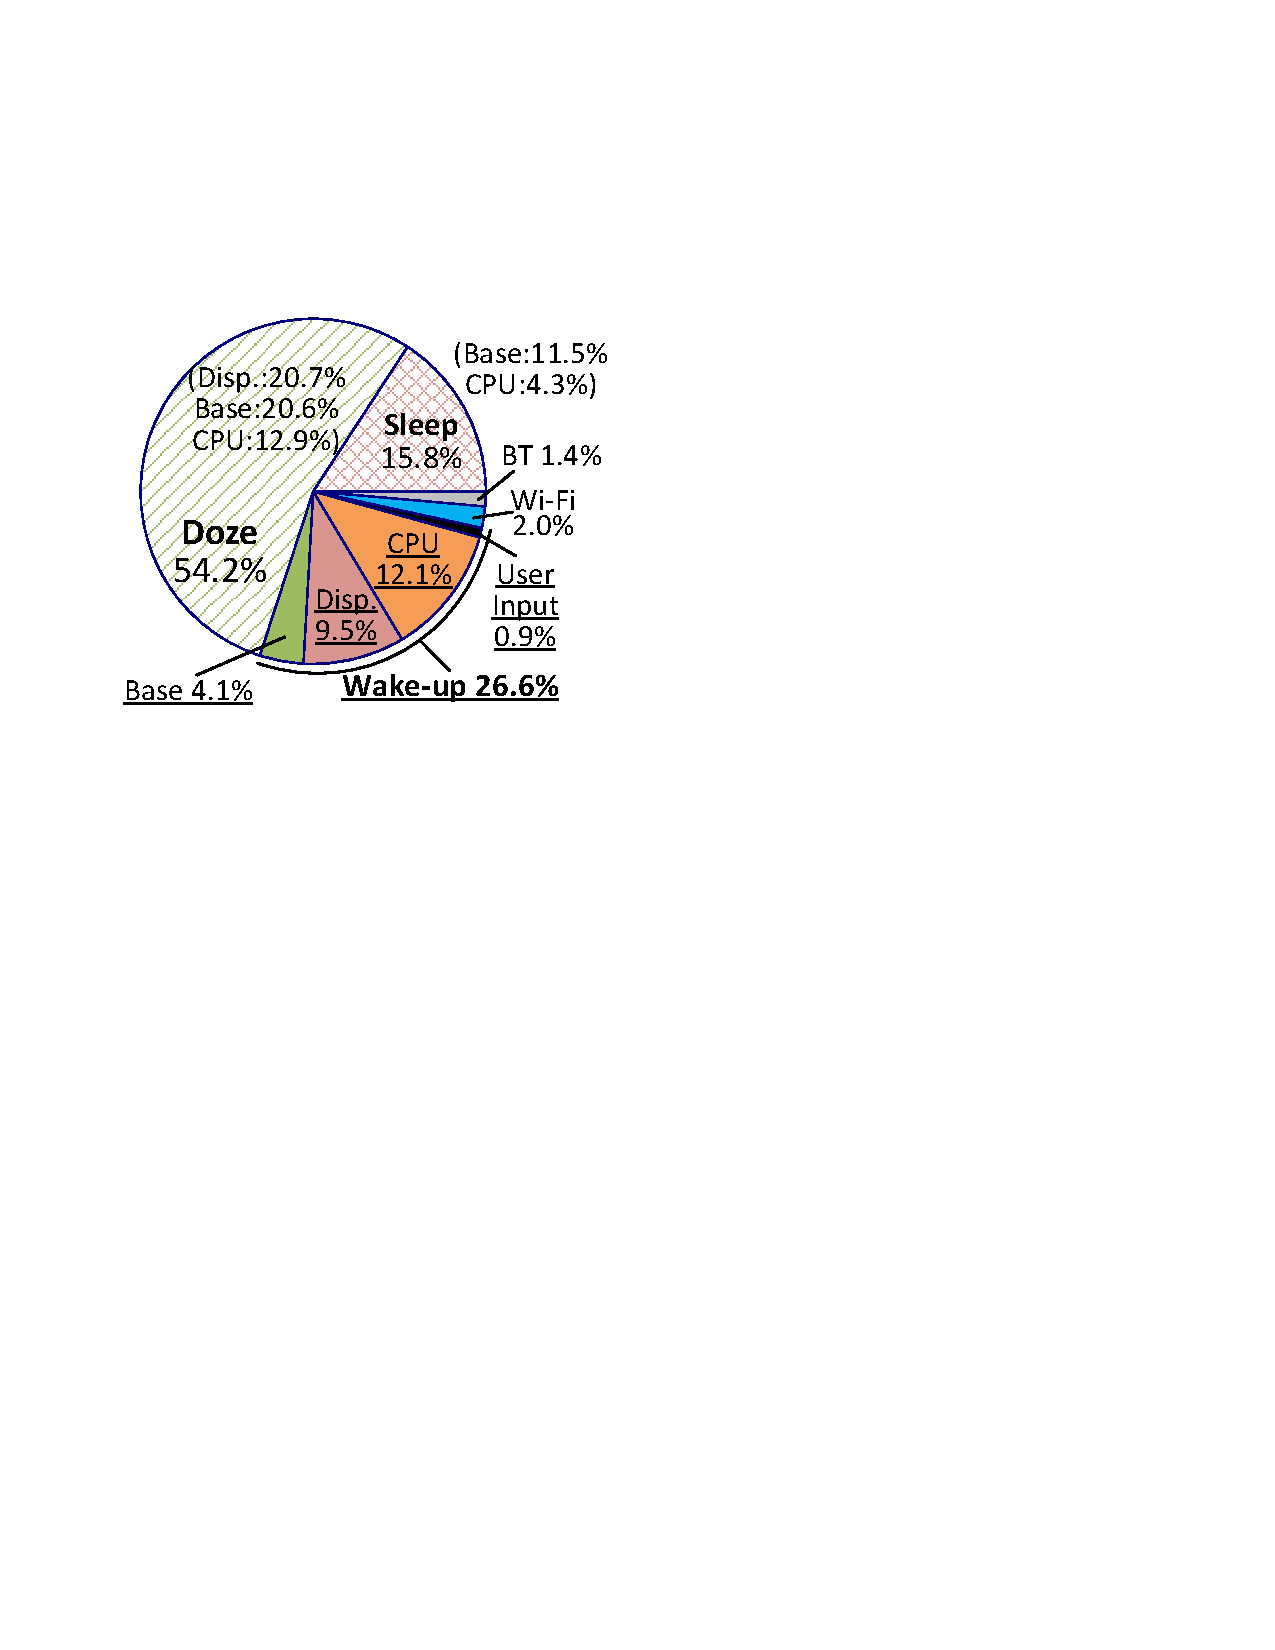
\includegraphics[width=.5\textwidth]{figs/smartwatch/energy_breakdown2.pdf} %\vspace{-2in}
	\caption{\footnotesize Component-level energy breakdown across all users.}
	\vspace{-.1in}
	\label{fig:energy}
\end{figure}

Figure~\ref{fig:energy} shows a more fine-grained energy breakdown. Within the dozing state, the energy consumed by the base, display, and CPU are roughly \{1.6:1.6:1\}. Despite its low brightness, display is still a key factor of battery drain when the watch is dozing. The dozing CPU energy comes from the maintenance window that periodically wakes up the CPU.
Within the awake state, display and CPU also dominate the energy consumption, accounting for 34.9\% and 44.5\% of the wake-up energy, respectively (or 9.5\% and 12.1\% of the overall energy respectively). The network incurs very small energy footprint (3.4\%). About 22\% of the Wi-Fi energy and 9\% of the Bluetooth energy are spent at the awake state (not shown in Figure~\ref{fig:energy}).

From Table~\ref{tab:model} and Figure~\ref{fig:energy}, we compute the average power consumption at the wakeup, dozing, and sleeping state to be 309.8mW, 31.9mW, and 14.5mW, respectively, across all users.
Note that the average dozing power (31.9mW) includes the base, the display, and the CPU power.
By weighing them using the usage duration breakdown, we can further compute the smartwatch's average power consumption to be 25.9mW across all states and users. Assuming that, a fully charged watch (with a battery capacity of 410 mAh for LG Urbane) can last for about 41.7 hours.


\section{Improving Smartwatch Energy Efficiency}
We study five methods for improving the smartwatch energy efficiency. We perform “what-if” analysis
on our dataset to reveal their impact on real smartwatch workloads
(or doing controlled experiments if a trace-driven analysis is not
feasible).

\textbf{1. Tuning the Awake$\rightarrow$Dozing Timer.} 

\textbf{2. Improving the Dozing$\rightarrow$Sleeping Mechanism.}

\textbf{3. Power-saving Color Transformation.}

\textbf{4. Bundling Delay-tolerant Push Notifications.} 

\textbf{5. Workload-aware CPU Configuration.}

Details for above 5 energy saving methods will be discussed during the proposal presentation.

%\chapter{Related Work} \label{chap:related}


\section{Live streaming and 360\degree{} video streaming}
First, to the best of our knowledge, few previous work, if any, have
measured or analyzed 360\degree{} live video streaming. However, there
is a large corpus of work in two related areas: \emph{personalized live streaming} and \emph{360\degree{} video streaming}.

\textbf{Living Streaming} broadcasts users themselves
and their surroundings using their (mobile) devices; viewers all
over the world can watch the live feed in real time. In 2016, two
papers~\cite{siekkinen2016first,wang2016anatomy} simultaneously studied Periscope and Meerkat, back
then the most popular platforms for personalized streaming on Android
and iOS mobile devices. Although different in their methodologies,
these two papers have a similar goal: shed some light on the
architecture (\emph{e.g.}, protocols and settings), the scale (\emph{e.g.}, the number
of broadcasters), and the performance (\emph{e.g.}, video quality and stalls)
of both streaming platforms. Our paper shares a similar goal but
in the context of 360\degree{} live video streaming offered by two different
platforms, YouTube and Facebook. Accordingly, our methodology in \lime
largely departs from the approaches proposed in~\cite{siekkinen2016first,wang2016anatomy}, as well
as our observations. Another recent paper~\cite{tang2016meerkat} studied the content and human
factors for Periscope and Meerkat.

Twitch is another popular platform for personalized live streaming,
with its primary focus on gaming broadcasting. Twitch differs
from Periscope and Meerkat since its broadcasters are mostly not
mobile. Pires \emph{et al}. \cite{pires2015youtube} were the first to look into Twitch (and
YouTube Live) back in 2015. Using a three-month dataset, they
showed the importance of Twitch with traffic peaks at more than
1 Tbps and millions of uploaded videos. Also in 2015, Zhang \emph{et al}. \cite{zhang2015crowdsourced} preliminarily investigated Twitch’s infrastructure using
both crawled data and captured traffic of local broadcasters/viewers.
More recently, Deng \emph{et al}. \cite{deng2017internet} expanded the latter study by exploring
Twitch’s infrastructure via a network of free proxies located
worldwide. They identified a geo-distributed infrastructure with
fine-grained server allocations, i.e., resources are dynamically allocated
to live streaming events based on their (growing) popularity.
There are also some earlier measurements on other live
streaming platforms such as live Internet TV and P2P live streaming
\cite{hei2007measurement,kaytoue2012watch,li2011measurement,silverston2007measuring,sripanidkulchai2004analysis}. The scope of \lime largely departs from them since we
focus on different content (360\degree{} live videos) and platforms (YouTube
and Facebook).

\textbf{360\degree{} Video Streaming} has become a hot research topic recently.
Researchers have investigated multiple aspects including projection/encoding methods \cite{kuzyakov2016next,kuzyakov2015under,lee2016rich360,nasrabadi2017adaptive,zhou2017measurement}, energy consumption \cite{jiang2017power},
viewport-adaptive streaming \cite{almquist2018prefetch,bao2016shooting,corbillon2017optimal,corbillon2017viewport,graf2017towards,petrangeli2017http,qian2016optimizing,qian2018flare,xiao2017optile,xie2017360probdash,xie2018cls},
cross-layer interaction \cite{sun2018multi,xie2017poi360}, and user experience \cite{broeck2017s}, \emph{etc}. Most
of the above studies focused on non-live 360\degree{} videos and none of
them investigated commercial 360\degree{} video streaming platforms as
we have done using crowd-sourcing.

In 2017, Afzal \emph{et al}. \cite{afzal2017characterization} studied the characteristics of (non-live)
360\degree{} videos uploaded to YouTube by simply searching for such
videos using keywords like ``360''. By analyzing a dataset of 4570
videos, they found that compared to regular videos, 360\degree{} videos
tend to be shorter, having higher resolutions, and more static (less
motion). \lime complements this effort since we focus on the
streaming performance rather than the 360\degree{} video characteristics. Furthermore, \lime investigates live streaming and expand our analysis
to Facebook as well.

In 2017, our positioning workshop paper
conducted a preliminary investigation of 360\degree{} live videos \cite{liu2017360}. \lime goes beyond \cite{liu2017360} by making several contributions: developing
a holistic measurement system for live videos, conducting crowdsourced
measurements for live 360\degree{} videos, and quantifying the
benefits of several key optimizations.

\section{Mobile VR}
In Chapter~\S\ref{chap:vr} we design and implement a multi-user mobile VR system \firefly. In literature relevant systems have been proposed, however they are all tested under certain single user scenarios, and there lack systematic study on its
multi-user counterpart.

\textbf{Single-user Mobile VR} has been well investigated in literature.
Furion \cite{lai2019furion} and Flashback \cite{boos2016flashback} demonstrate
high-quality single-user VR on COTS smartphones.
MoVR \cite{abari2016cutting,abari2017enabling} employs 60 GHz mmWave wireless for mobile
VR. Liu \emph{et al.} \cite{liu2018cutting} proposed system-level optimizations
for the mobile VR rendering pipeline. Tan \emph{et al.} explored supporting
mobile VR over LTE \cite{tan2018vr}. None of the above work
explicitly focuses on the multi-user scenario.

\textbf{Multi-user VR/AR}. Despite a plethora of work on single user
VR, much fewer studies have been conducted on
multi-user environment. The most relevant work to \firefly is
MUVR \cite{li2018muvr} which can only be simulated to support 4 concurrent VR users.
Bao \emph{et al.} developed
a multi-user 360° video streaming system based on
multicast \cite{bao2017motion}. A recent positioning paper \cite{liu2019supporting} discusses several
practical issues of designing a multi-user VR system
(without system implementation). Some studies investigated
multi-user or collaborative augmented reality (AR) \cite{qiu2018avr,ran2019sharear,zhang2018cars}.
Compared to the above work, \firefly is a generic multi-user
VR system. It achieves much better scalability compared to
MUVR.


\section{Characterizing Android Wear OS}

\textbf{Mobile devices ``in the wild''}. Researchers have carried out numerous
crowd-sourced measurements of smartphones~\cite{huang10,falaki10_mobisys,shepard10,phonelab,qian12_mobisys,rosen15_imc,nikravesh15_mobisys,chen15:sigmetrics}. While they partially motivate our smartwatch user study, much fewer efforts have been made for wearable devices.
Among them,
Gouveia \etal studied how users engage with activity trackers~\cite{gouveia15_ubicomp}.
%
Lazar \etal interviewed 17 participants to study the incentives of using and abandoning smart devices~\cite{lazar15_ubicomp}.
%
Lyons studied usage practices of traditional dumb watches by conducting a user survey~\cite{lyons15_iswc}.
%
Min \etal characterized smartwatch battery use based on online survey and a user study involving 17 users~\cite{min15_iswc}. They studied users' satisfaction toward smartwatch life, charging behaviors,
and interaction patterns.
%
In a recent extended abstract~\cite{poyraz_iiswc16}, Poyraz \etal also described their smartwatch user study involving 32 users for 70 days. Using the collected data, they analyzed the watches' power consumption and characterized user activities. While the detailed data collection and measurement methodologies were not fully documented, many of their findings such as the active state's high energy contribution compared to its short usage duration are qualitatively similar to ours.
%
Compared to~\cite{min15_iswc} and~\cite{poyraz_iiswc16}, we instead investigate a much wider spectrum of characteristics such as push notification, app usage, and network traffic by leveraging a much richer set of data items collected in Table~\ref{tab:data}.

\textbf{Android Wear OS}. Recently, Liu \etal analyzed the execution of Android Wear OS and presented a series of inefficiencies and OS implications~\cite{liu16_mobisys,liu15_apsys}.
Compared to its in-lab, controlled experiments, our study on Android smartwatch contributes the understanding of real-world wearable usage as well as the entailed design implications -- backed by more solid evidence.
Furthermore, our study characterizes key system aspects that were missing in the prior work, most notably power modeling and network behaviors.

\textbf{Other wearable system and applications} have also been studied in literature.
LiKamWa \etal characterized the energy consumption of Google Glass~\cite{likamwa13_apsys}.
%
Huang \etal proposed a fast storage system for wearables based on battery-backed RAM and offloading~\cite{huang15_atc}.
%
Santagati \etal designed an ultrasonic networking framework for wearable
medical devices~\cite{santagati15_mobisys}.
%
Miao \etal investigated the implications of smartwatches' circular display on resource usage~\cite{miao16_hotmobile}.
%
Ham \etal proposed a novel display energy conservation scheme for wearables~\cite{ham15_atc}.
%
There also exists a large body of work from the mobile computing, sensing, and HCI community. These studies focus on novel wearable applications~\cite{shen16_mobisys, nirjon15_mobisys,mayberry14_mobisys}, wearable user interface design~\cite{chen14_chi, plaumann16_iswc}, and wearable security~\cite{wang15_mobicom, liu15_ccs}.
%
In contrast, our smartwatch measurement focuses on characterizing wearable user behavior, application usage, energy consumption, and network traffic -- all in the wild.



\chapter{Conclusion and Future Work} \label{chap:conc}

\section{Future Work}
.


\begin{singlespace}
\bibliographystyle{aiaa}
\bibliography{./tex/thesis-bib,xing,robustnet,multipath_feng,smartwatch,./lime_bib/360,./lime_bib/biblio}
\end{singlespace}

\end{document}
